%KernelSemanticsChapter.tex

\chapter{Kernel Semantics}\label{chap:kernelsemantics}
%\ksec{8.4.4 Kernel Semantics}

\ksec{Kernel Semantics Overview (KerML 8.4.4.1)}

\pn The semantics of constructs in the Kernel Layer are specified in terms of the foundational constructs defined in the Core layer, extended with \lang~Logic for time-varying operation of systems.  \lang~Logic is introduced in \S\ref{sec:modallogic} and elaborated in Appendix \ref{chapter:KL}.

%The Kernel Semantic Model Library (see 9.2) extends the mathematically-specified to provide a rich set of pre-declared elements and relationships, which can be tailored, as needed by users.


%The Metamath program verifies all proofs in \texttt{set.mm} in about 3 s.

\subsection{\logicid~ Logic}\label{sec:modallogic}


\pn Classical logic and set theory are used to define a many-world modal logic with a Kripke structure (see Appendix \ref{chapter:KL}).

\pn A \bemph{modal logic} defines symbols whose meaning differs depending in which ``world" the symbol is evaluated.

\pn A \bemph{temporal logic} is a modal logic for which each world corresponds to an instant or interval of time.
%A good synopsis of other temporal logics used can be found in \cite{Konur-2013}, which surveys 18 of them.  

\begin{restatable}{definition}{dfmodel}~\blTitle{df-model}~ 
A dynamic architecture model, $\mathfrak{M}$ is defined as a tuple
 
\begin{align}
\vdash \mathfrak{M}
  \equiv \langle \mathbf{T}, \prec, D, E, P, \mathbf{I} \rangle \label{eq:df-model}\tag{df-model}
\end{align}
 
  such that
 
$\mathbf{T}$: is a set of time instants, 

$\prec$: is a temporal precedence relation, 

$D$: is a design expressed in KerML,

$E$: is a selected KerML element in the design to be modeled $E \in D$, 

$P(\tau)$: is the system boundary at time $\tau \in \mathbf{T}$, and

$\mathbf{I}\lsem d,\tau\rsem$: is an interpretation for design element $d\in D$ at time $\tau \in \mathbf{T}$.
\end{restatable}

\pn $E$ will be treated as a set theory \bemph{class}:  a collection defined by a rule.

\pn The interpretation $\mathbf{I}\lsem E,\tau\rsem$ finds an element (member) of $E$ (if there is one) for any $\tau \in \mathbf{T}$.

\pn $E$ may have many possible elements at time $\tau$; interpretation picks just one.

%If $E$ is empty for any $\tau \in \mathbf{T}$, it is \bemph{unsatisfiable}, so has some kind of fundamental error.

\pn $P(\tau)$ is the system boundary where the system interacts with its environment.  It is called \bemph{P} in honor of the Parnas four variable model to represent the physical world sensors detect and actuators affect.  When modeling subsystems, $P$ represents the inputs and outputs of connected subsystems.

\pn Constructing a model $\mathfrak{M}$  for $E$ is \bemph{execution}.


\pn The interpretation $\mathbf{I}\lsem d,\tau\rsem$ is only defined for any element $d$ in the design $D$.
Furthermore, the interpretation is contingent on the values of the system boundary $P(\tau)$.

\pn \texttt{Type} and  \texttt{Classifier} elements have the same interpretation for all $\tau\in\mathbf{T}$, because they are immutable.  \texttt{Class} elements may have variable features, and lifetimes.

%\pn For this several definitions will be useful.

\begin{restatable}{leandefinition}{Model}~\leanTitle{Model}~ Define a dynamic architecture model in Lean, as a
\texttt{structure} bundling $D$/$E$/$P$/$\mathbf{I}$. $\mathbf{T}$ and $\prec$ are \emph{not} separate fields
here: this file already treats \texttt{TIME}/$\prec$ as global, ambient primitives rather than something that
varies per model (matching how \texttt{SFS.mm}'s own \texttt{ctime}/\texttt{wtp} are likewise bare, file-level
constants, not parameters to anything) --- a \texttt{Model} field for them would just rename what's already
there. The book states $E\in D$ on first introduction, then immediately reinterprets $E$ itself as a
\emph{class} (``$E$ will be treated as a set theory class: a collection defined by a rule''; ``$E$ may have
many possible elements at time $\tau$; interpretation picks just one''). The second reading is the one
formalized here (\texttt{E\_sub\_D} : $E\subseteq D$, not $E\in D$), since it's the one under which
``interpretation picks one member of $E$'' is meaningful at all; the first-stated $E\in D$ is not separately
restated as an axiom.

\texttt{\textcolor{leancolor}{structure} \textcolor{leanyellow}{Model} \textcolor{leancolor}{where}}

\texttt{~~D : Set Element}

\texttt{~~E : Set Element}

\texttt{~~E\_sub\_D : E $\subseteq$ D}

\texttt{~~P : Time $\to$ Set Element}

\texttt{~~I : Element $\to$ TVal (Set Element)}
\label{Model}
\end{restatable}

\pn  $\mathbf{I}\lsem d \rsem$ is the same at every time $\tau\in\mathbf{T}$:
 
 \begin{restatable}{definition}{dfblmodels}~\blTitle{df-bl.models}~ Define interpretation of predicate for
any $\tau \in \mathbf{T}$
\begin{align}
\vdash \tau \in \mathbf{T}\quad\Rightarrow\quad \vdash ( \mathbf{I} \lsem
    \mw{\varphi} \rsem \rightarrow \mathbf{I} \lsem \mw{\varphi} , \tau \rsem
    )\label{eq:df-bl.models}\tag{df-bl.models}
\end{align}
\end{restatable}

\begin{restatable}{leantheorem}{axDlModelsLean}~\leanTitle{ax\_dl\_models}~ Define interpretation of predicate
for any $\tau\in\mathbf{T}$, in Lean. The $\tau\in\mathbf{T}$ hypothesis \texttt{SFS.mm} carries is no longer
stated separately: it's automatic from \texttt{t0}'s type (\texttt{Time}, not bare \texttt{Instant}).

\texttt{\textcolor{leancolor}{theorem} \textcolor{leanyellow}{ax\_dl\_models} \{$\varphi$ : TProp\} \{t0 : Time\} : interp $\varphi$ $\to$ interpAt $\varphi$ t0 := fun h $\Rightarrow$ h t0}
\label{ax_dl_models}
\end{restatable}

\begin{restatable}{definition}{dfblmodelsc}~\blTitle{df-bl.modelsc}~ Define interpretation of values over
any $\tau \in \mathbf{T}$
\begin{align}
\vdash \tau \in \mathbf{T}\quad\Rightarrow\quad \vdash ( \mathbf{I} \lsem
    \mc{A} \rsem = \mc{B} \rightarrow \mathbf{I} \lsem \mc{A} , \tau \rsem =
    \mc{B} )\label{eq:df-bl.modelsc}\tag{df-bl.modelsc}
\end{align}
\end{restatable}

\pn \texttt{df-bl.modelsc} is only meaningful when $\mc{A}$ is actually constant, and is not needed to make
any of the value-side distribution facts in \texttt{SFS.lean} provable --- so, unlike everything else in this
section, it is deliberately \emph{not} restated as a Lean axiom or theorem.


\pn $\mathbf{T}$ is the set of real times between 0 and $\mathsf{\mc{now}}$, inclusive:

\begin{restatable}{definition}{dfbltime}~\blTitle{df-bl.time}~ Define domain of time $\mathbf{T}$
from $\msc{t} = 0$ to $\mathsf{\mc{now}}$.
\begin{align}
\vdash \mathbf{T} = \{ \msc{x}~\vert~( \msc{x} \in \mathbb{R} \wedge 0 \le \msc{x}
    \wedge \msc{x} \le \mathsf{\mc{now}} )
    \}\label{eq:df-bl.time}\tag{df-bl.time}
\end{align}
\end{restatable}

\begin{restatable}{leandefinition}{TIMELean}~\leanTitle{TIME}~ Define domain of time $\mathbf{T}$ in Lean, as
\texttt{Set.Icc 0 now} (Mathlib's own closed-interval notation) rather than a raw set-builder --- the same
content, but already equipped with Mathlib's interval lemmas.

\texttt{\textcolor{leancolor}{def} \textcolor{leanyellow}{TIME} : Set Instant := Set.Icc 0 now}
\label{TIME}
\end{restatable}

\pn Define the \bemph{present instant} $\mathsf{\mc{now}}$:

\begin{restatable}{definition}{dfblnowrr}~\blTitle{df-bl.nowrr}~ now is a non-negative real number.
\begin{align}
\vdash ( \mathsf{\mc{now}} \in \mathbb{R} \wedge 0 \le \mathsf{\mc{now}}
    )\label{eq:df-bl.nowrr}\tag{df-bl.nowrr}
\end{align}
\end{restatable}

\begin{restatable}{leandefinition}{nowLean}~\leanTitle{now}~ Define the present instant in Lean:
class-based (2026-08-26), the simplest instance of the general repair recipe (\S\ref{sec:model} above,
\texttt{Lifetimes}) -- \texttt{now} needs no guard the way \texttt{birth}/\texttt{death}/\texttt{timeof}
did (``does a nonnegative real exist'' is trivially true, witnessed by $0$ itself), so
\texttt{Classical.choice} alone is enough to build a real model, no new axiom needed.

\texttt{\textcolor{leancolor}{class} \textcolor{leanyellow}{Now} \textcolor{leancolor}{where}}

\texttt{~~now : $\mathbb{R}$}

\texttt{~~now\_nonneg : 0 $\le$ now}

\texttt{\textcolor{leancolor}{export} Now (now now\_nonneg)}

\texttt{\textcolor{leancolor}{noncomputable instance} \textcolor{leanyellow}{nowModel} : Now :=}

\texttt{~~$\langle$Classical.choose (\ldots), Classical.choose\_spec (\ldots)$\rangle$}
\label{now}
\end{restatable}


\pn Define \bemph{temporal precedence}.  (Note the subtle difference between $\prec$ and $<$):

\begin{restatable}{definition}{dfblbefore}~\blTitle{df-bl.before}~ Temporal Precedence (before).
\begin{align}
\vdash ( ( \tau_1 \in \mathbf{T} \wedge \tau_2 \in \mathbf{T} ) \rightarrow (
    \tau_1 \prec \tau_2 \leftrightarrow \tau_1 < \tau_2 )
    )\label{eq:df-bl.before}\tag{df-bl.before}
\end{align}
\end{restatable}

\begin{restatable}{leandefinition}{tprec}~\leanTitle{tprec}~ Define temporal precedence in Lean, directly as
$<$ on all of $\mathbb{R}$ rather than only characterized on \texttt{TIME}. Its Leibniz congruence
(\texttt{bl.tpeq1}/\texttt{bl.tpeq2} in \texttt{SFS.mm} --- needed there as \emph{extra} axioms because
\texttt{wtp} is a bare primitive) is just \texttt{congrArg}, free of charge here.

\texttt{\textcolor{leancolor}{def} \textcolor{leanyellow}{tprec} (t1 t2 : Instant) : Prop := t1 < t2}

\texttt{\textcolor{leancolor}{infix:50} " $\prec$ " => tprec}
\label{tprec}
\end{restatable}

\begin{restatable}{leantheorem}{dlBefore}~\leanTitle{dl\_before}~ Temporal Precedence (before), in Lean ---
free directly from \texttt{tprec}'s own definition.

\texttt{\textcolor{leancolor}{theorem} \textcolor{leanyellow}{dl\_before} \{t1 t2 : Instant\} (\_ : t1 $\in$ TIME) (\_ : t2 $\in$ TIME) :}

\texttt{~~(t1 $\prec$ t2) $\leftrightarrow$ t1 < t2 := Iff.rfl}
\label{dl_before}
\end{restatable}

\pn It's also useful to define ``before or coincident":

\begin{restatable}{definition}{dfblbeforeeq}~\blTitle{df-bl.beforeeq}~ Temporal Precedence (before or
coincident).
\begin{align}
\vdash ( ( \tau_1 \in \mathbf{T} \wedge \tau_2 \in \mathbf{T} ) \rightarrow (
    \tau_1 \preccurlyeq \tau_2 \leftrightarrow ( \tau_1 < \tau_2 \vee \tau_1 =
    \tau_2 ) ) )\label{eq:df-bl.beforeeq}\tag{df-bl.beforeeq}
\end{align}
\end{restatable}

\begin{restatable}{leandefinition}{tprecEq}~\leanTitle{tprecEq}~ Define ``before or coincident'' in Lean,
directly as $\le$ on all of $\mathbb{R}$, same reasoning as \texttt{tprec} above.

\texttt{\textcolor{leancolor}{def} \textcolor{leanyellow}{tprecEq} (t1 t2 : Instant) : Prop := t1 $\le$ t2}

\texttt{\textcolor{leancolor}{infix:50} " $\preccurlyeq$ " => tprecEq}
\label{tprecEq}
\end{restatable}

\begin{restatable}{leantheorem}{dlBeforeeq}~\leanTitle{dl\_beforeeq}~ Temporal Precedence (before or
coincident), in Lean --- free directly from \texttt{tprecEq}'s own definition (\texttt{le\_iff\_lt\_or\_eq}).

\texttt{\textcolor{leancolor}{theorem} \textcolor{leanyellow}{dl\_beforeeq} \{t1 t2 : Instant\} (\_ : t1 $\in$ TIME) (\_ : t2 $\in$ TIME) :}

\texttt{~~(t1 $\preccurlyeq$ t2) $\leftrightarrow$ (t1 < t2 $\vee$ t1 = t2) := le\_iff\_lt\_or\_eq}
\label{dl_beforeeq}
\end{restatable}

\pn Beyond precedence itself, \texttt{SFS.lean} builds the full apparatus that \texttt{interp}/\texttt{interpAt} (already used silently above, in \ref{ax_dl_models}) rest on: the temporal-value/-predicate domains, the untimed (``always'', the modal $\Box$) and timed readings of both, and a family of soundness results about how far each ordinary logical connective can be pulled through the untimed reading.

\pn Two small witnessing facts about $\mathbf{T}$ are used throughout what follows: $0$ and $\mathsf{\mc{now}}$ are both always members of $\mathbf{T}$.

\begin{restatable}{leantheorem}{TIMEnonemptyNowt}~\leanTitle{TIME\_nonempty / dl\_nowt}~ $\mathbf{T}$ is nonempty (witnessed by $0$), and $\mathsf{\mc{now}}$ is itself always a member of $\mathbf{T}$, in Lean.

\texttt{\textcolor{leancolor}{theorem} \textcolor{leanyellow}{TIME\_nonempty} : (0 : Instant) $\in$ TIME := $\langle$le\_refl 0, now\_nonneg$\rangle$}

\texttt{\textcolor{leancolor}{theorem} \textcolor{leanyellow}{dl\_nowt} : now $\in$ TIME := $\langle$now\_nonneg, le\_refl now$\rangle$}
\label{TIME_nonempty}
\label{dl_nowt}
\end{restatable}

\pn Temporal values and predicates are evaluated over an instant \emph{together with} a proof that it lies in $\mathbf{T}$, not a bare instant:

\begin{restatable}{leandefinition}{TimeTValTProp}~\leanTitle{Time / TVal / TProp}~ \texttt{Time} is the subtype of instants carrying their own \texttt{TIME}-membership proof. A \bemph{temporal value} (\texttt{TVal}) is one plain value per instant --- what \texttt{SFS.mm}'s $\mc{A}$ denotes when read as varying with the world; a \bemph{temporal predicate} (\texttt{TProp}) is a function from instants to truth values --- \texttt{SFS.mm}'s $\mw{\varphi}$, read the same way. Everything below is stated against \texttt{Time}, not bare \texttt{Instant}.

\texttt{\textcolor{leancolor}{abbrev} \textcolor{leanyellow}{Time} := $\uparrow$TIME}

\texttt{\textcolor{leancolor}{abbrev} \textcolor{leanyellow}{TVal} ($\alpha$ : Type*) := Time $\to$ $\alpha$}

\texttt{\textcolor{leancolor}{abbrev} \textcolor{leanyellow}{TProp} := Time $\to$ Prop}
\label{Time}
\label{TVal}
\label{TProp}
\end{restatable}

\begin{restatable}{leandefinition}{InterpInterpAt}~\leanTitle{interp / interpAt}~ \texttt{SFS.mm}'s $\mathbf{I}\lsem\mw{\varphi},\tau\rsem$ (interpretation at a specific instant) is definitionally just application, since \texttt{TProp} already \emph{is} ``value at each instant''; \texttt{SFS.mm}'s $\mathbf{I}\lsem\mw{\varphi}\rsem$ (the untimed/``always'' reading) holds when $\varphi$ holds at every instant --- the standard modal necessity ($\Box$) reading, the only one consistent with \texttt{SFS.mm}'s own commentary that tautologies are ``things true at every instant.''

\texttt{\textcolor{leancolor}{def} \textcolor{leanyellow}{interpAt} ($\varphi$ : TProp) (t0 : Time) : Prop := $\varphi$ t0}

\texttt{\textcolor{leancolor}{def} \textcolor{leanyellow}{interp} ($\varphi$ : TProp) : Prop := $\forall$ t, $\varphi$ t}
\label{interpAt}
\label{interp}
\end{restatable}

\pn A plain (non-temporally-varying) fact --- an ordinary \texttt{Prop}, or a bare equality/membership --- can always be read as a temporal one, embedded via the constant function; the following are soundness/congruence facts about that embedding.

\begin{restatable}{leantheorem}{ConstantEmbeddingProp}~\leanTitle{ax\_dl\_taut / dl\_ty / dl\_tyt / ax\_dl\_bi}~ \texttt{ax\_dl\_taut} (\texttt{SFS.mm} \texttt{ax-bl.taut}): a plain fact, embedded as a constant \texttt{TProp}, is trivially \texttt{interp}-true once any instant exists (\ref{TIME_nonempty} guarantees one). \texttt{dl\_ty} (\texttt{SFS.mm} \texttt{bl.ty}) is the same argument for set membership. \texttt{dl\_tyt} (\texttt{SFS.mm} \texttt{bl.tyt}) is its timed counterpart, trivial both ways since \texttt{interpAt} is literal evaluation. \texttt{ax\_dl\_bi} (\texttt{SFS.mm} \texttt{ax-bl.bi}) is the same reading for a bare biconditional between two ordinary \texttt{Prop}s; \texttt{SFS.mm}'s $\tau_1,\tau_2\in\mathbf{T}$ hypotheses are automatic here from \texttt{t1 t2 : Time}.

\texttt{\textcolor{leancolor}{theorem} \textcolor{leanyellow}{ax\_dl\_taut} \{p : Prop\} : p $\to$ interp (\textcolor{leancolor}{fun} (\_ : Time) $\Rightarrow$ p) := \textcolor{leancolor}{fun} h \_ $\Rightarrow$ h}

\texttt{\textcolor{leancolor}{theorem} \textcolor{leanyellow}{dl\_ty} \{$\alpha$\} \{A : $\alpha$\} \{B : Set $\alpha$\} : A $\in$ B $\to$ interp (\textcolor{leancolor}{fun} (\_ : Time) $\Rightarrow$ A $\in$ B) := ax\_dl\_taut}

\texttt{\textcolor{leancolor}{theorem} \textcolor{leanyellow}{dl\_tyt} \{$\alpha$\} \{A : $\alpha$\} \{B : Set $\alpha$\} \{t0 : Time\} :}

\texttt{~~A $\in$ B $\leftrightarrow$ interpAt (\textcolor{leancolor}{fun} \_ $\Rightarrow$ A $\in$ B) t0 := Iff.rfl}

\texttt{\textcolor{leancolor}{theorem} \textcolor{leanyellow}{ax\_dl\_bi} \{p q : Prop\} \{t1 t2 : Time\} (\_ : t1 = t2) :}

\texttt{~~(p $\leftrightarrow$ q) $\leftrightarrow$ (interpAt (\textcolor{leancolor}{fun} (\_ : Time) $\Rightarrow$ p) t1 $\leftrightarrow$ interpAt (\textcolor{leancolor}{fun} (\_ : Time) $\Rightarrow$ q) t2) := Iff.rfl}
\label{ax_dl_taut}
\label{dl_ty}
\label{dl_tyt}
\label{ax_dl_bi}
\end{restatable}

\begin{restatable}{leandefinition}{InterpValFamily}~\leanTitle{interpValAt / interpVal / ax\_dl\_eq}~ \texttt{interpValAt}/\texttt{interpVal} are the value-side counterparts of \texttt{interpAt}/\texttt{interp} --- timed is literal evaluation, untimed is anchored at instant $0$ (\ref{TIME_nonempty}). Unlike predicate-\texttt{interp} this is not a $\forall$-aggregation, so it commutes with every pointwise-defined value operator unconditionally. \texttt{ax\_dl\_eq} (\texttt{SFS.mm} \texttt{ax-bl.eq}) is the value-level counterpart of \texttt{ax\_dl\_bi}, same constant-embedding reading.

\texttt{\textcolor{leancolor}{def} \textcolor{leanyellow}{interpValAt} \{$\alpha$\} (A : TVal $\alpha$) (t0 : Time) : $\alpha$ := A t0}

\texttt{\textcolor{leancolor}{def} \textcolor{leanyellow}{interpVal} \{$\alpha$\} (A : TVal $\alpha$) : $\alpha$ := A $\langle$0, TIME\_nonempty$\rangle$}

\texttt{\textcolor{leancolor}{theorem} \textcolor{leanyellow}{ax\_dl\_eq} \{$\alpha$\} \{A B : $\alpha$\} \{t1 t2 : Time\} (\_ : t1 = t2) :}

\texttt{~~(A = B) $\leftrightarrow$ (interpValAt (\textcolor{leancolor}{fun} (\_ : Time) $\Rightarrow$ A) t1 = interpValAt (\textcolor{leancolor}{fun} (\_ : Time) $\Rightarrow$ B) t2) := Iff.rfl}
\label{interpValAt}
\label{interpVal}
\label{ax_dl_eq}
\end{restatable}

\pn The existential duals of the closed/open-interval universal-quantification facts documented above (\ref{dl_alldd}, \ref{dl_allcd}, \ref{dl_allcc}, \ref{dl_alldc}) are all instances of one generic classical fact, proved once rather than four times:

\begin{restatable}{leantheorem}{ExistsDualFamily}~\leanTitle{exists\_iff\_not\_forall\_not / dl\_exdd / dl\_excc / dl\_excd / dl\_exdc}~ \texttt{exists\_iff\_not\_forall\_not} is plain classical De Morgan, nothing interval-specific about it; \texttt{dl\_exdd}/\texttt{dl\_excc}/\texttt{dl\_excd}/\texttt{dl\_exdc} (\texttt{SFS.mm} \texttt{bl.exdd}/\texttt{bl.excc}/\texttt{bl.excd}/\texttt{bl.exdc}) instantiate it at the closed, open, open-right, and open-left intervals in turn; unlike their universal counterparts their $\tau_1,\tau_2$ stay plain \texttt{Instant}s, matching \texttt{SFS.mm}'s own (hypothesis-free) statement of them.

\texttt{\textcolor{leancolor}{theorem} \textcolor{leanyellow}{exists\_iff\_not\_forall\_not} \{D : Type*\} (P : D $\to$ Prop) : ($\exists$ x, P x) $\leftrightarrow$ $\neg$ $\forall$ x, $\neg$ P x}

\texttt{\textcolor{leancolor}{theorem} \textcolor{leanyellow}{dl\_exdd} (t1 t2 : Instant) ($\varphi$ : TProp) :}

\texttt{~~($\exists$ x : Time, x.val $\in$ Set.Icc t1 t2 $\wedge$ $\varphi$ x) $\leftrightarrow$ $\neg$ $\forall$ x : Time, $\neg$ (x.val $\in$ Set.Icc t1 t2 $\wedge$ $\varphi$ x) :=}

\texttt{~~exists\_iff\_not\_forall\_not \_}

\texttt{\textcolor{leancolor}{theorem} \textcolor{leanyellow}{dl\_excc} (t1 t2 : Instant) ($\varphi$ : TProp) :}

\texttt{~~($\exists$ x : Time, x.val $\in$ Set.Ioo t1 t2 $\wedge$ $\varphi$ x) $\leftrightarrow$ $\neg$ $\forall$ x : Time, $\neg$ (x.val $\in$ Set.Ioo t1 t2 $\wedge$ $\varphi$ x) :=}

\texttt{~~exists\_iff\_not\_forall\_not \_}

\texttt{\textcolor{leancolor}{theorem} \textcolor{leanyellow}{dl\_excd} (t1 t2 : Instant) ($\varphi$ : TProp) :}

\texttt{~~($\exists$ x : Time, x.val $\in$ Set.Ioc t1 t2 $\wedge$ $\varphi$ x) $\leftrightarrow$ $\neg$ $\forall$ x : Time, $\neg$ (x.val $\in$ Set.Ioc t1 t2 $\wedge$ $\varphi$ x) :=}

\texttt{~~exists\_iff\_not\_forall\_not \_}

\texttt{\textcolor{leancolor}{theorem} \textcolor{leanyellow}{dl\_exdc} (t1 t2 : Instant) ($\varphi$ : TProp) :}

\texttt{~~($\exists$ x : Time, x.val $\in$ Set.Ico t1 t2 $\wedge$ $\varphi$ x) $\leftrightarrow$ $\neg$ $\forall$ x : Time, $\neg$ (x.val $\in$ Set.Ico t1 t2 $\wedge$ $\varphi$ x) :=}

\texttt{~~exists\_iff\_not\_forall\_not \_}
\label{exists_iff_not_forall_not}
\label{dl_exdd}
\label{dl_excc}
\label{dl_excd}
\label{dl_exdc}
\end{restatable}

\pn The timed connectives lift ordinary logical operators pointwise to \texttt{TProp}, each with its own infix notation:

\begin{restatable}{leandefinition}{TimedConnectives}~\leanTitle{tand / tor / tnot / timp / tiff}~ Pointwise-defined timed conjunction, disjunction, negation, implication, and biconditional --- every ``\texttt{interpAt} distributes over connective $X$'' fact is then \texttt{Iff.rfl}, since \texttt{interpAt} is literal evaluation and every combinator here is defined pointwise.

\texttt{\textcolor{leancolor}{def} \textcolor{leanyellow}{tand} ($\varphi$ $\psi$ : TProp) : TProp := \textcolor{leancolor}{fun} t $\Rightarrow$ $\varphi$ t $\wedge$ $\psi$ t}

\texttt{\textcolor{leancolor}{def} \textcolor{leanyellow}{tor} ($\varphi$ $\psi$ : TProp) : TProp := \textcolor{leancolor}{fun} t $\Rightarrow$ $\varphi$ t $\vee$ $\psi$ t}

\texttt{\textcolor{leancolor}{def} \textcolor{leanyellow}{tnot} ($\varphi$ : TProp) : TProp := \textcolor{leancolor}{fun} t $\Rightarrow$ $\neg$ $\varphi$ t}

\texttt{\textcolor{leancolor}{def} \textcolor{leanyellow}{timp} ($\varphi$ $\psi$ : TProp) : TProp := \textcolor{leancolor}{fun} t $\Rightarrow$ $\varphi$ t $\to$ $\psi$ t}

\texttt{\textcolor{leancolor}{def} \textcolor{leanyellow}{tiff} ($\varphi$ $\psi$ : TProp) : TProp := \textcolor{leancolor}{fun} t $\Rightarrow$ $\varphi$ t $\leftrightarrow$ $\psi$ t}

\texttt{\textcolor{leancolor}{infixr:70} " $\wedge_t$ " => tand}

\texttt{\textcolor{leancolor}{infixr:65} " $\vee_t$ " => tor}

\texttt{\textcolor{leancolor}{prefix:75} "$\neg_t$" => tnot}

\texttt{\textcolor{leancolor}{infixr:60} " $\to_t$ " => timp}

\texttt{\textcolor{leancolor}{infix:55} " $\leftrightarrow_t$ " => tiff}
\label{tand}
\label{tor}
\label{tnot}
\label{timp}
\label{tiff}
\end{restatable}

\pn Under the necessity ($\Box$) reading, \texttt{interp} distributes over $\wedge_t$/$\forall$ both ways, but --- as with any normal modal box operator --- only \emph{one} direction is valid for $\vee_t$/$\neg_t$/$\to_t$/$\leftrightarrow_t$/$\exists$ in general (the classic K-axiom asymmetry). \texttt{SFS.mm} states its own \texttt{df-bl.or}/\texttt{df-bl.not}/\texttt{df-bl.im}/\texttt{df-bl.bi}/\texttt{bl.ex} as full, unconditional biconditionals; \texttt{SFS.lean} proves only the sound direction of each, witnessing the unsound direction false in general via two-instant counterexamples (not restated as axioms).

\begin{restatable}{leantheorem}{dlAn}~\leanTitle{dl\_an}~ \texttt{SFS.mm} \texttt{df-bl.an} (untimed): sound, \texttt{interp} distributes over $\wedge_t$ both ways (\texttt{forall\_and}).

\texttt{\textcolor{leancolor}{theorem} \textcolor{leanyellow}{dl\_an} ($\varphi$ $\psi$ : TProp) : interp ($\varphi$ $\wedge_t$ $\psi$) $\leftrightarrow$ (interp $\varphi$ $\wedge$ interp $\psi$) := forall\_and}
\label{dl_an}
\end{restatable}

\begin{restatable}{leantheorem}{dlAl}~\leanTitle{dl\_al}~ \texttt{SFS.mm} \texttt{df-bl.al} (untimed universal-quantification exportation): sound, swapping two $\forall$s is always valid.

\texttt{\textcolor{leancolor}{theorem} \textcolor{leanyellow}{dl\_al} \{D : Type*\} ($\varphi$ : D $\to$ TProp) :}

\texttt{~~interp (\textcolor{leancolor}{fun} t $\Rightarrow$ $\forall$ x, $\varphi$ x t) $\leftrightarrow$ $\forall$ x, interp ($\varphi$ x) := forall\_comm}
\label{dl_al}
\end{restatable}

\begin{restatable}{leantheorem}{dlAnThree}~\leanTitle{dl\_3an}~ \texttt{SFS.mm} \texttt{bl.3an} (untimed, three terms): a direct corollary of \ref{dl_an} applied to the flat right-associated shape, not a fresh axiom.

\texttt{\textcolor{leancolor}{theorem} \textcolor{leanyellow}{dl\_3an} ($\varphi$ $\psi$ ch : TProp) : interp ($\varphi$ $\wedge_t$ $\psi$ $\wedge_t$ ch) $\leftrightarrow$ (interp $\varphi$ $\wedge$ interp $\psi$ $\wedge$ interp ch)}
\label{dl_3an}
\end{restatable}

\begin{restatable}{leantheorem}{dlDfrexTwo}~\leanTitle{dl\_dfrex2}~ \texttt{SFS.mm} \texttt{bl.dfrex2} (untimed): unlike \ref{dl_ex_sound} below, this one \emph{is} sound both ways --- it compares \texttt{interp} of two \emph{pointwise}-equivalent \texttt{TProp}s ($\exists x\in A,\varphi\,x\,t$ and $\neg\forall x\in A,\neg\varphi\,x\,t$ are classically equivalent for every fixed $t$, no swap of $\forall t$ past $\exists x$ involved), so it is a congruence fact, not a K-axiom-asymmetry one.

\texttt{\textcolor{leancolor}{theorem} \textcolor{leanyellow}{dl\_dfrex2} \{D : Type*\} (A : Set D) ($\varphi$ : D $\to$ TProp) :}

\texttt{~~interp (\textcolor{leancolor}{fun} t $\Rightarrow$ $\exists$ x $\in$ A, $\varphi$ x t) $\leftrightarrow$ interp (\textcolor{leancolor}{fun} t $\Rightarrow$ $\neg$ $\forall$ x $\in$ A, $\neg$ $\varphi$ x t)}
\label{dl_dfrex2}
\end{restatable}

\begin{restatable}{leantheorem}{dlOrSound}~\leanTitle{dl\_or\_sound}~ \texttt{SFS.mm} \texttt{df-bl.or} (untimed), sound direction only. The converse is \bemph{false} in general: witnessed on \texttt{TIME} as soon as it has two distinct instants $\tau_1\ne\tau_2$, by $\varphi := (\cdot=\tau_1)$, $\psi := (\cdot=\tau_2)$ --- $\varphi\vee_t\psi$ holds at every instant in $\{\tau_1,\tau_2\}$ but neither disjunct holds at both.

\texttt{\textcolor{leancolor}{theorem} \textcolor{leanyellow}{dl\_or\_sound} ($\varphi$ $\psi$ : TProp) : (interp $\varphi$ $\vee$ interp $\psi$) $\to$ interp ($\varphi$ $\vee_t$ $\psi$)}
\label{dl_or_sound}
\end{restatable}

\begin{restatable}{leantheorem}{dlThreeOrSound}~\leanTitle{dl\_3or\_sound}~ \texttt{SFS.mm} \texttt{bl.3or} (untimed, three terms), sound direction only --- same asymmetry as \ref{dl_or_sound}, one level deeper.

\texttt{\textcolor{leancolor}{theorem} \textcolor{leanyellow}{dl\_3or\_sound} ($\varphi$ $\psi$ ch : TProp) :}

\texttt{~~(interp $\varphi$ $\vee$ interp $\psi$ $\vee$ interp ch) $\to$ interp ($\varphi$ $\vee_t$ $\psi$ $\vee_t$ ch)}
\label{dl_3or_sound}
\end{restatable}

\begin{restatable}{leantheorem}{dlNotSound}~\leanTitle{dl\_not\_sound}~ \texttt{SFS.mm} \texttt{df-bl.not} (untimed), sound direction only: if $\varphi$ fails at every instant it certainly doesn't hold at every instant. The converse is \bemph{false} in general, same asymmetry as \ref{dl_or_sound}.

\texttt{\textcolor{leancolor}{theorem} \textcolor{leanyellow}{dl\_not\_sound} ($\varphi$ : TProp) : interp ($\neg_t$$\varphi$) $\to$ $\neg$ interp $\varphi$ :=}

\texttt{~~\textcolor{leancolor}{fun} h hall $\Rightarrow$ h $\langle$0, TIME\_nonempty$\rangle$ (hall $\langle$0, TIME\_nonempty$\rangle$)}
\label{dl_not_sound}
\end{restatable}

\begin{restatable}{leantheorem}{dlImSound}~\leanTitle{dl\_im\_sound}~ \texttt{SFS.mm} \texttt{df-bl.im} (untimed), sound direction only (the modal K-axiom shape itself). The converse fails by the same shape as \ref{dl_or_sound}.

\texttt{\textcolor{leancolor}{theorem} \textcolor{leanyellow}{dl\_im\_sound} ($\varphi$ $\psi$ : TProp) : interp ($\varphi$ $\to_t$ $\psi$) $\to$ (interp $\varphi$ $\to$ interp $\psi$) :=}

\texttt{~~\textcolor{leancolor}{fun} h h$\varphi$ t $\Rightarrow$ h t (h$\varphi$ t)}
\label{dl_im_sound}
\end{restatable}

\begin{restatable}{leantheorem}{dlBiSound}~\leanTitle{dl\_bi\_sound}~ \texttt{SFS.mm} \texttt{df-bl.bi} (untimed), sound direction only, same asymmetry as \ref{dl_or_sound}/\ref{dl_not_sound}/\ref{dl_im_sound}.

\texttt{\textcolor{leancolor}{theorem} \textcolor{leanyellow}{dl\_bi\_sound} ($\varphi$ $\psi$ : TProp) : interp ($\varphi$ $\leftrightarrow_t$ $\psi$) $\to$ (interp $\varphi$ $\leftrightarrow$ interp $\psi$) :=}

\texttt{~~\textcolor{leancolor}{fun} h $\Rightarrow$ $\langle$\textcolor{leancolor}{fun} h$\varphi$ t $\Rightarrow$ (h t).mp (h$\varphi$ t), \textcolor{leancolor}{fun} h$\psi$ t $\Rightarrow$ (h t).mpr (h$\psi$ t)$\rangle$}
\label{dl_bi_sound}
\end{restatable}

\begin{restatable}{leantheorem}{dlExSound}~\leanTitle{dl\_ex\_sound}~ \texttt{SFS.mm} \texttt{bl.dfrex2}/\texttt{bl.ex} (untimed existential exportation), sound direction only. The converse is the classic invalid $\forall\exists$-to-$\exists\forall$ swap: different instants may need different witnesses.

\texttt{\textcolor{leancolor}{theorem} \textcolor{leanyellow}{dl\_ex\_sound} \{D : Type*\} ($\varphi$ : D $\to$ TProp) :}

\texttt{~~($\exists$ x, interp ($\varphi$ x)) $\to$ interp (\textcolor{leancolor}{fun} t $\Rightarrow$ $\exists$ x, $\varphi$ x t) :=}

\texttt{~~\textcolor{leancolor}{fun} $\langle$x, hx$\rangle$ t $\Rightarrow$ $\langle$x, hx t$\rangle$}
\label{dl_ex_sound}
\end{restatable}

\begin{restatable}{leantheorem}{dlRaltRext}~\leanTitle{dl\_ralt / dl\_rext}~ \texttt{SFS.mm} \texttt{df-bl.ralt}/\texttt{df-bl.rext}, timed restricted universal/existential quantification: both \texttt{Iff.rfl}, same reason every other timed fact is --- \texttt{interpAt} is literal evaluation.

\texttt{\textcolor{leancolor}{theorem} \textcolor{leanyellow}{dl\_ralt} \{D : Type*\} ($\varphi$ : D $\to$ TProp) (A : Set D) (t0 : Time) :}

\texttt{~~interpAt (\textcolor{leancolor}{fun} t $\Rightarrow$ $\forall$ x $\in$ A, $\varphi$ x t) t0 $\leftrightarrow$ $\forall$ x, x $\in$ A $\to$ interpAt ($\varphi$ x) t0 := Iff.rfl}

\texttt{\textcolor{leancolor}{theorem} \textcolor{leanyellow}{dl\_rext} \{D : Type*\} ($\varphi$ : D $\to$ TProp) (A : Set D) (t0 : Time) :}

\texttt{~~interpAt (\textcolor{leancolor}{fun} t $\Rightarrow$ $\exists$ x $\in$ A, $\varphi$ x t) t0 $\leftrightarrow$ $\exists$ x, x $\in$ A $\wedge$ interpAt ($\varphi$ x) t0 := Iff.rfl}
\label{dl_ralt}
\label{dl_rext}
\end{restatable}

\pn Temporal values also support pointwise-lifted relations, matching \texttt{SFS.mm}'s \texttt{df-bl.eq}/\texttt{df-bl.eqt}/\texttt{df-bl.lt}/\texttt{df-bl.ltt}/\texttt{df-bl.am}/\texttt{df-bl.amt}:

\begin{restatable}{leandefinition}{TeqTltTle}~\leanTitle{teq / tlt / tle}~ Pointwise equality, less-than, and less-or-equal between two \texttt{TVal $\mathbb{R}$}s.

\texttt{\textcolor{leancolor}{def} \textcolor{leanyellow}{teq} (A B : TVal $\mathbb{R}$) : TProp := \textcolor{leancolor}{fun} t $\Rightarrow$ A t = B t}

\texttt{\textcolor{leancolor}{def} \textcolor{leanyellow}{tlt} (A B : TVal $\mathbb{R}$) : TProp := \textcolor{leancolor}{fun} t $\Rightarrow$ A t < B t}

\texttt{\textcolor{leancolor}{def} \textcolor{leanyellow}{tle} (A B : TVal $\mathbb{R}$) : TProp := \textcolor{leancolor}{fun} t $\Rightarrow$ A t $\le$ B t}
\label{teq}
\label{tlt}
\label{tle}
\end{restatable}

\begin{restatable}{leantheorem}{dlBitrit}~\leanTitle{dl\_bitrit}~ \texttt{SFS.mm} \texttt{bl.bitrit}: transitivity of timed $\Box$-biconditional --- literally \texttt{Iff.trans}, not a fresh fact, since \texttt{interpAt} is just evaluation.

\texttt{\textcolor{leancolor}{theorem} \textcolor{leanyellow}{dl\_bitrit} \{$\varphi$ $\psi$ ch : TProp\} \{t0 : Time\} (h1 : interpAt ($\varphi$ $\leftrightarrow_t$ $\psi$) t0)}

\texttt{~~(h2 : interpAt ($\psi$ $\leftrightarrow_t$ ch) t0) : interpAt ($\varphi$ $\leftrightarrow_t$ ch) t0 := h1.trans h2}
\label{dl_bitrit}
\end{restatable}

%\subsection{Existence}

\pn KerML classes may not exist\index{ex@\texttt{ex}} for the whole duration of the system as a whole.  Define a predicate $\texttt{ex}(c,\tau)$ that returns true if class $c$ exists (is not empty $\emptyclass$) at time $\tau$ and false otherwise.
The interpretation of a classifier which doesn't exist is the empty class, $\emptyclass$.

\begin{restatable}{definition}{dfexists}~\blTitle{df-bl.exists}~ Define element existence predicate
\begin{align}
\vdash (~ \texttt{ex}(c,\tau) \leftrightarrow \mathbf{I}\lsem c,\tau\rsem\neq\emptyclass~)
\label{eq:df-bl.exists}\tag{df-bl.exists}
\end{align}
\end{restatable}

\begin{restatable}{leandefinition}{existsAtLean}~\leanTitle{existsAt}~ Define element existence predicate in
Lean, for an \texttt{Occurrence} (\texttt{TVal (Set Item)}, so ``$\ne\emptyset$'' reads directly against its
own \texttt{interpValAt}).

\texttt{\textcolor{leancolor}{def} \textcolor{leanyellow}{existsAt} (A : Occurrence) (t0 : Time) : Prop := interpValAt A t0 $\ne$ $\emptyset$}
\label{existsAt}
\end{restatable}

\pn The \textidx{birth}\index{birth@\texttt{birth}} time of a KerML class $\texttt{birth}(c)$ is when it comes into existence.  The birth of $c$ is $\tau_b$ if-and-only-if $c$ exists at
$\tau_b$ and does not exist before $\tau_b$.
%The death time of a classifier $\texttt{death}(c)$ is when it ceases to exist.

\begin{restatable}{definition}{dfbirth}~\blTitle{df-bl.birth}~Define Birth time.
\begin{align}
\vdash (~\texttt{birth}(c)=\tau_b \leftrightarrow ( \texttt{ex}(c,\tau_b) \wedge \forall \tau \in (0[,)\tau_b)~\vert~ \lnot \texttt{ex}(c,\tau)~)~)
\label{eq:df-bl.birth}\tag{df-bl.birth}
\end{align}
\end{restatable}

\pn \texttt{birth}, \texttt{death}, and \texttt{timeof} (\S\ref{sec:timeof} below) are defined together in
Lean, class-based (2026-08-26), porting a general repair recipe from toy \texttt{$\mathbb{N}$} to the real
\texttt{Instant}/\texttt{Time}/\texttt{TIME}: guard each characterizing law with its presupposition, keep the
function total (or here \texttt{Option}-valued) with an unconstrained/undefined value when the presupposition
fails, then \emph{prove} a model exists rather than assume one. The port is not mechanical -- \texttt{$\mathbb{N}$}
is well-ordered for free, so any nonempty subset has a least element with no extra assumption; an arbitrary
subset of the dense continuum \texttt{Time} need not (e.g.\ $\{t \mid t.\mathrm{val} < 0.5\}$ has an infimum but
no attained minimum) -- so \texttt{birth}'s (and \texttt{timeof}'s) guard needs some further structural fact
the $\mathbb{N}$ case gets for free from well-ordering. That fact is \ref{hasFirstTick} (below), built directly
on \ref{finitePartition}'s finite shared-tick structure -- not, as originally (until 2026-08-26), a
separately-axiomatized \texttt{hasFirstInstant} asserting (falsely, in general, for a dense order) that
\emph{every} satisfiable predicate has an attained least witness. \texttt{death} needs no such extra fact at
all: its guard is self-certifying, the same reasoning that already justified \texttt{endShot}'s
\texttt{Option} redesign.

\begin{restatable}{leandefinition}{LifetimesLean}~\leanTitle{Lifetimes}~ Define the \texttt{birth}/\texttt{death}/
\texttt{timeof} class in Lean: \texttt{birth}/\texttt{timeof} stay total (\texttt{startShot} stays mandatory;
\texttt{timeof}'s own guard is analogous), \texttt{death} stays \texttt{Option}-valued (\texttt{endShot} does
not); \texttt{birthIff}/\texttt{timeofIff} are guarded on existing/holding somewhere (unconditional would force
even a never-existing \texttt{A} or nowhere-true $\varphi$ to have \emph{some} first instant); \texttt{deathIff}
needs no such guard -- the \texttt{Option} codomain already \emph{is} the guard.

\texttt{\textcolor{leancolor}{class} \textcolor{leanyellow}{Lifetimes} \textcolor{leancolor}{where}}

\texttt{~~birth : Occurrence $\to$ Time}

\texttt{~~death : Occurrence $\to$ Option Time}

\texttt{~~birthIff : $\forall$ \{A : Occurrence\} \{t0 : Time\}, ($\exists$ s, existsAt A s) $\to$}

\texttt{~~~~(birth A = t0 $\leftrightarrow$ existsAt A t0 $\wedge$ $\forall$ t1 : Time, t1.val $\in$ Set.Ico (0 : Instant) t0.val $\to$ $\lnot$ existsAt A t1)}

\texttt{~~deathIff : $\forall$ \{A : Occurrence\} \{t0 : Time\},}

\texttt{~~~~death A = some t0 $\leftrightarrow$ existsAt A t0 $\wedge$ $\forall$ t1 : Time, t1.val $\in$ Set.Ioc t0.val now $\to$ $\lnot$ existsAt A t1}

\texttt{~~timeof : TProp $\to$ Time}

\texttt{~~timeofIff : $\forall$ \{$\varphi$ : TProp\} \{t1 : Time\}, ($\exists$ s, interpAt $\varphi$ s) $\to$}

\texttt{~~~~(timeof $\varphi$ = t1 $\leftrightarrow$ interpAt $\varphi$ t1 $\wedge$ $\forall$ t : Time, t.val $\in$ Set.Ico (0 : Instant) t1.val $\to$ $\lnot$ interpAt $\varphi$ t)}

\texttt{\textcolor{leancolor}{export} Lifetimes (birth death birthIff deathIff timeof timeofIff)}
\label{Lifetimes}
\end{restatable}

\begin{restatable}{leantheorem}{hasFirstTickLean}~\leanTitle{hasFirstTick}~ \texttt{Time}'s dense order gives
no well-ordering on its own (\texttt{\{t $\mid$ 0 < t.val\}} has an infimum but no attained minimum), so this
reformation still needs \emph{some} structural fact ruling that out -- but not a fresh axiom: \ref{finitePartition}
(broadened, above) already says \texttt{P (d $\cdot$)} can only ever change value at a shared tick, so a finite
search over \texttt{Fin (tickCount + 1)} suffices (via \texttt{Finset.min'} over the finitely many
witnessing ticks, using an auxiliary \texttt{ticks\_bucket} lemma -- every instant's \texttt{d}-value matches
the \texttt{d}-value at the largest shared tick $\le$ it). Retires the separately-axiomatized
\texttt{hasFirstInstant} this reformation used to need (2026-08-26). Stated generically (not fixed to
\texttt{existsAt A}) so it serves both \texttt{birth} (\texttt{d := A}, \texttt{P := ($\cdot \ne \emptyset$)})
and \texttt{timeof} below (\texttt{d := $\varphi$}, \texttt{P := id}) without a near-duplicate theorem for
each. Proof omitted here.

\texttt{\textcolor{leancolor}{theorem} \textcolor{leanyellow}{hasFirstTick} \{$\alpha$ : Type\} (d : TVal $\alpha$) (P : $\alpha$ $\to$ Prop)}

\texttt{~~(h : $\exists$ s : Time, P (d s)) : $\exists$ $\tau$, IsLeast \{t : Time $\mid$ P (d t)\} $\tau$}
\label{hasFirstTick}
\end{restatable}

\begin{restatable}{leantheorem}{birthExistsLean}~\leanTitle{birth\_exists}~ A total selector satisfying
\texttt{birthIff}'s guarded spec exists for every occurrence: \ref{hasFirstTick}'s witness (at
\texttt{d := A}, \texttt{P := ($\cdot \ne \emptyset$)}) when \texttt{A} exists somewhere, an unconstrained
junk value otherwise. Proof omitted here (case split on existence, direct from \ref{hasFirstTick} in the
positive case).

\texttt{\textcolor{leancolor}{theorem} \textcolor{leanyellow}{birth\_exists} (A : Occurrence) :}

\texttt{~~$\exists$ t0 : Time, ($\exists$ s, existsAt A s) $\to$}

\texttt{~~~~(existsAt A t0 $\wedge$ $\forall$ t1 : Time, t1.val $\in$ Set.Ico (0 : Instant) t0.val $\to$ $\lnot$ existsAt A t1)}
\label{birth_exists}
\end{restatable}

\begin{restatable}{leantheorem}{deathExistsLean}~\leanTitle{death\_exists}~ A total selector satisfying
\texttt{deathIff}'s guarded spec exists for every occurrence, \texttt{none} when no greatest existence instant
exists -- pure classical logic, \emph{no} extra axiom needed (unlike \texttt{birth\_exists}): the guarded
hypothesis, when it holds, already hands over a witness satisfying \texttt{IsGreatest} directly (existence set
membership together with ``nothing exists strictly after $t0$'' is exactly \texttt{IsGreatest} of the
existence set at $t0$), so no well-ordering-style assumption about \texttt{Occurrence} is ever needed. Proof
omitted here (case split on whether a greatest existence instant exists, uniqueness via
\texttt{IsGreatest.unique}).

\texttt{\textcolor{leancolor}{theorem} \textcolor{leanyellow}{death\_exists} (A : Occurrence) :}

\texttt{~~$\exists$ d : Option Time, $\forall$ t0 : Time, d = some t0 $\leftrightarrow$}

\texttt{~~~~(existsAt A t0 $\wedge$ $\forall$ t1 : Time, t1.val $\in$ Set.Ioc t0.val now $\to$ $\lnot$ existsAt A t1)}
\label{death_exists}
\end{restatable}

\begin{restatable}{leantheorem}{timeofExistsLean}~\leanTitle{timeof\_exists}~ SFS.mm \texttt{df-bl.timeof}'s own
guarded existence (\S\ref{sec:timeof}), exactly \ref{birth_exists}'s argument with \texttt{existsAt A} replaced
by \texttt{interpAt $\varphi$} -- the same structural shape (\texttt{timeofIff} is \texttt{birthIff} with
\texttt{interpAt $\varphi$} in place of \texttt{existsAt A}), so the same proof, via the same generic
\ref{hasFirstTick} (\texttt{d := $\varphi$}, \texttt{P := id}), carries over unchanged.

\texttt{\textcolor{leancolor}{theorem} \textcolor{leanyellow}{timeof\_exists} ($\varphi$ : TProp) :}

\texttt{~~$\exists$ t1 : Time, ($\exists$ s, interpAt $\varphi$ s) $\to$}

\texttt{~~~~(interpAt $\varphi$ t1 $\wedge$ $\forall$ t : Time, t.val $\in$ Set.Ico (0 : Instant) t1.val $\to$ $\lnot$ interpAt $\varphi$ t)}
\label{timeof_exists}
\end{restatable}

\begin{restatable}{leandefinition}{modelLean}~\leanTitle{model}~ The consistency certificate: a real model,
built via \texttt{Classical.choose} over \ref{birth_exists}/\ref{death_exists}/\ref{timeof_exists} -- exactly
the construction that would be impossible without \texttt{birthIff}/\texttt{deathIff}/\texttt{timeofIff}'s
guards. A plain (not locally-scoped) \texttt{instance}, so every downstream use of
\texttt{birth}/\texttt{death}/\texttt{birthIff}/\texttt{deathIff}/\texttt{timeof}/\texttt{timeofIff} elsewhere
resolves to it automatically. \texttt{birthIff}/\texttt{deathIff}/\texttt{timeofIff}'s own field proofs (via
\texttt{Classical.choose\_spec} and a short order-theoretic argument) are omitted here for brevity. The audit,
matching the toy \texttt{$\mathbb{N}$} demo's own convention: \texttt{\#print axioms model} reports exactly
Lean's three standard classical axioms plus the project's pre-existing foundational primitives plus
\emph{one} new ingredient, \ref{finitePartition} -- not for well-ordering (dense \texttt{Time} still has none),
but because \ref{hasFirstTick} (reused for both \texttt{birth} and \texttt{timeof}) needs \emph{some}
structural fact ruling out an unattained infimum, and \texttt{finitePartition}'s finite shared-tick structure
supplies it (2026-08-26, retiring the earlier, separately-axiomatized \texttt{hasFirstInstant}) -- nothing
else.

\texttt{\textcolor{leancolor}{noncomputable instance} \textcolor{leanyellow}{model} : Lifetimes \textcolor{leancolor}{where}}

\texttt{~~birth A := Classical.choose (birth\_exists A)}

\texttt{~~death A := Classical.choose (death\_exists A)}

\texttt{~~timeof $\varphi$ := Classical.choose (timeof\_exists $\varphi$)}

\texttt{~~birthIff \{A\} \{t0\} h := \textcolor{leancolor}{by} \ldots}

\texttt{~~deathIff \{A\} \{t0\} := \textcolor{leancolor}{by} \ldots}

\texttt{~~timeofIff \{$\varphi$\} \{t1\} h := \textcolor{leancolor}{by} \ldots}
\label{model}
\end{restatable}

\pn $(0[,)\tau_b)$ is the open-right time interval\index{ xdc@\lstinline+.,+ open right} from time 0 up to, but not including $\tau_b$:

\begin{restatable}{lemma}{blalldc}~\blTitle{bl.alldc}~ Universal quantification over open-right
time interval [t1 ., t2].
\begin{align}
\vdash ( \tau_1 \in \mathbf{T} \wedge \tau_2 \in \mathbf{T}
    )\quad\Rightarrow\quad \vdash ( \forall \msc{x} \in \mathbf{T} ( \msc{x}
    \in ( \tau_1 [,) \tau_2 ) \wedge \mw{\varphi} ) \leftrightarrow \forall
    \msc{x} \in \mathbf{T} ( \tau_1 \le \msc{x} \wedge \msc{x} < \tau_2 \wedge
    \mw{\varphi} ) )\label{eq:bl.alldc}\tag{bl.alldc}
\end{align}
\end{restatable}

\begin{restatable}{leantheorem}{dlAlldc}~\leanTitle{dl\_alldc}~ Universal quantification over open-right time
interval, in Lean --- just unfolds what membership in an open-right interval means arithmetically, already
exactly Mathlib's \texttt{Set.mem\_Ico}.

\texttt{\textcolor{leancolor}{theorem} \textcolor{leanyellow}{dl\_alldc} (t1 t2 : Time) ($\varphi$ : TProp) :}

\texttt{~~($\forall$ x : Time, x.val $\in$ Set.Ico t1.val t2.val $\wedge$ $\varphi$ x) $\leftrightarrow$}

\texttt{~~~~($\forall$ x : Time, t1.val $\le$ x.val $\wedge$ x.val < t2.val $\wedge$ $\varphi$ x)}
\label{dl_alldc}
\end{restatable}

\pn The \textidx{death}\index{death@\texttt{death}} time of a KerML class $\texttt{death}(c)$ is its last moment of existence.  The death of $c$ is $\tau_d$ if-and-only-if $c$ exists at
$\tau_d$ and does not exist after $\tau_d$.

\begin{restatable}{definition}{dfdeath}~\blTitle{df-bl.death}~Define Death time.
\begin{align}
\vdash (~\texttt{death}(c)=\tau_d \leftrightarrow ( \texttt{ex}(c,\tau_d) \wedge \forall \tau \in (\tau_d(,]\mathsf{\mc{now}})~\vert~ \lnot \texttt{ex}(c,\tau)~)~)
\label{eq:df-bl.death}\tag{df-bl.death}
\end{align}
\end{restatable}

\pn \texttt{death} is \texttt{Option}-valued in Lean (\ref{Lifetimes} above, 2026-08-25/26):
\texttt{Occurrences.kerml}'s own \texttt{endShot: Instant[0..1]} means an occurrence may not have ended by
\texttt{now}. A total \texttt{death} forced every occurrence, including one that never exists, to have
\emph{some} death instant -- inconsistent, the same defect \S\ref{sec:bldefinedness} generalizes and fixes.
\texttt{death} itself stays exactly this way -- partial, faithful to \texttt{endShot}'s own cardinality. Allen's
intervals below (\S\ref{sec:allen}) are re-expressed in terms of a separate, \emph{total} reading instead
(\ref{effectiveEnd}): "active-now" occurrences are simply treated as ending at \texttt{now} itself.

\pn $(\tau_d(,]\mathsf{\mc{now}})$ is the open-left\index{ xcd@\lstinline+,.+ open left} time interval greater than time $\tau_d$ up to $\mathsf{\mc{now}}$.

\begin{restatable}{lemma}{blallcd}~\blTitle{bl.allcd}~ Universal quantification over open-left
time interval [t1 ,. t2].
\begin{align}
\vdash ( \tau_1 \in \mathbf{T} \wedge \tau_2 \in \mathbf{T}
    )\quad\Rightarrow\quad \vdash ( \forall \msc{x} \in \mathbf{T} ( \msc{x}
    \in ( \tau_1 (,] \tau_2 ) \wedge \mw{\varphi} ) \leftrightarrow \forall
    \msc{x} \in \mathbf{T} ( \tau_1 < \msc{x} \wedge \msc{x} \le \tau_2 \wedge
    \mw{\varphi} ) )\label{eq:bl.allcd}\tag{bl.allcd}
\end{align}
\end{restatable}

\begin{restatable}{leantheorem}{dlAllcd}~\leanTitle{dl\_allcd}~ Universal quantification over open-left time
interval, in Lean --- Mathlib's \texttt{Set.mem\_Ioc}.

\texttt{\textcolor{leancolor}{theorem} \textcolor{leanyellow}{dl\_allcd} (t1 t2 : Time) ($\varphi$ : TProp) :}

\texttt{~~($\forall$ x : Time, x.val $\in$ Set.Ioc t1.val t2.val $\wedge$ $\varphi$ x) $\leftrightarrow$}

\texttt{~~~~($\forall$ x : Time, t1.val < x.val $\wedge$ x.val $\le$ t2.val $\wedge$ $\varphi$ x)}
\label{dl_allcd}
\end{restatable}

\pn The lifetime of a KerML class  $\texttt{life}(c)$\index{life@\texttt{life}} is the closed time interval between birth and death.

\begin{restatable}{definition}{dflifetime}~\blTitle{df-bl.lifetime}~Define Lifetime.
\begin{align}
\vdash \texttt{life}(c)~=~ (\texttt{birth}(c)~[,]~\texttt{death}(c))
\label{eq:df-bl.lifetime}\tag{df-bl.lifetime}
\end{align}
\end{restatable}

\begin{restatable}{leandefinition}{lifeLean}~\leanTitle{life}~ Define Lifetime in Lean, as \texttt{Set.Icc}
between \texttt{birth}'s and \texttt{effectiveEnd}'s own values (\ref{effectiveEnd}) -- total, unlike
\texttt{SFS.mm}'s own \texttt{df-lifetime} (\eqref{eq:df-bl.lifetime} above), which is left unchanged, still
in terms of raw \texttt{death}.

\texttt{\textcolor{leancolor}{noncomputable def} \textcolor{leanyellow}{life} (A : Occurrence) : Set Instant := Set.Icc (birth A).val (effectiveEnd A).val}
\label{life}
\end{restatable}

\pn $[,]$ denotes an interval closed\index{ xdd@\lstinline+..+ closed both} on both ends;
$(,)$ denotes and interval open\index{ xcc@\lstinline+,,+ open both}  on both ends.

\begin{restatable}{lemma}{blalldd}~\blTitle{bl.alldd}~ Universal quantification over closed time
interval [t1 .. t2].
\begin{align}
\vdash ( \tau_1 \in \mathbf{T} \wedge \tau_2 \in \mathbf{T}
    )\quad\Rightarrow\quad \vdash ( \forall \msc{x} \in \mathbf{T} ( \msc{x}
    \in ( \tau_1 [,] \tau_2 ) \wedge \mw{\varphi} ) \leftrightarrow \forall
    \msc{x} \in \mathbf{T} ( \tau_1 \le \msc{x} \wedge \msc{x} \le \tau_2
    \wedge \mw{\varphi} ) )\label{eq:bl.alldd}\tag{bl.alldd}
\end{align}
\end{restatable}
\index{ xdd@\lstinline+..+ closed interval}

\begin{restatable}{leantheorem}{dlAlldd}~\leanTitle{dl\_alldd}~ Universal quantification over closed time
interval, in Lean --- Mathlib's \texttt{Set.mem\_Icc}.

\texttt{\textcolor{leancolor}{theorem} \textcolor{leanyellow}{dl\_alldd} (t1 t2 : Time) ($\varphi$ : TProp) :}

\texttt{~~($\forall$ x : Time, x.val $\in$ Set.Icc t1.val t2.val $\wedge$ $\varphi$ x) $\leftrightarrow$}

\texttt{~~~~($\forall$ x : Time, t1.val $\le$ x.val $\wedge$ x.val $\le$ t2.val $\wedge$ $\varphi$ x)}
\label{dl_alldd}
\end{restatable}

\begin{restatable}{lemma}{blallcc}~\blTitle{bl.allcc}~ Universal quantification over open time
interval [t1 ,, t2].
\begin{align}
\vdash ( \tau_1 \in \mathbf{T} \wedge \tau_2 \in \mathbf{T}
    )\quad\Rightarrow\quad \vdash ( \forall \msc{x} \in \mathbf{T} ( \msc{x}
    \in ( \tau_1 (,) \tau_2 ) \wedge \mw{\varphi} ) \leftrightarrow \forall
    \msc{x} \in \mathbf{T} ( \tau_1 < \msc{x} \wedge \msc{x} < \tau_2 \wedge
    \mw{\varphi} ) )\label{eq:bl.allcc}\tag{bl.allcc}
\end{align}
\end{restatable}

\begin{restatable}{leantheorem}{dlAllcc}~\leanTitle{dl\_allcc}~ Universal quantification over open time
interval, in Lean --- Mathlib's \texttt{Set.mem\_Ioo}.

\texttt{\textcolor{leancolor}{theorem} \textcolor{leanyellow}{dl\_allcc} (t1 t2 : Time) ($\varphi$ : TProp) :}

\texttt{~~($\forall$ x : Time, x.val $\in$ Set.Ioo t1.val t2.val $\wedge$ $\varphi$ x) $\leftrightarrow$}

\texttt{~~~~($\forall$ x : Time, t1.val < x.val $\wedge$ x.val < t2.val $\wedge$ $\varphi$ x)}
\label{dl_allcc}
\end{restatable}
\index{ xcc@\lstinline+,,+ open interval}

\subsection{Instant and Interval}

For \logicid ~Logic, time is defined in an independent \texttt{Domain} library package.
The fundamental element of time is \texttt{Instant}\index{instant} with which \texttt{Interval}\index{interval} is defined.

\ecaption{Instant and Interval}
\begin{lstlisting}
  type Instant specializes TimeValue {
    doc /* an instant of time */
  }

  classifier Interval
  {
    doc /* an interval is a duration between two instants */
    feature lowerBound : Instant;
    feature upperBound : Instant;
    feature openLeft : Boolean;
    feature openRight : Boolean; 
    inv {lowerBound <= upperBound}   
  }
\end{lstlisting}

\subsection{Allen's Intervals}\label{sec:allen}

\pn KerML Class lifetimes can be related using Allen's intervals\index{Allen's intervals} in \ref{table:allensintervals}.  

\begin{table}[h]
\caption{Allen's Intervals}
\begin{center}
\begin{tabular}{|c|c|c|c|}
\hline
\textbf{Relation} & \textbf{Interpretation} & \textbf{Formula} & \textbf{Predicate} \\ \hline
$X < Y$ & X \bemph{precedes} Y & $\texttt{effectiveEnd}(X) \prec \texttt{birth}(Y)$ & \textidx{precedes}(X,Y) \\ \hline
$X ~m~ Y$ & X  \bemph{meets} Y & $\texttt{effectiveEnd}(X) = \texttt{birth}(Y)$ & \textidx{meets}(X,Y) \\ \hline
$X ~o~ Y$ & X  \bemph{overlaps} Y & $\texttt{birth}(Y)\prec \texttt{effectiveEnd}(X)$ & \textidx{overlaps}(X,Y) \\ \hline
$X ~s~ Y$ & X  \bemph{starts} Y & $\texttt{birth}(X) = \texttt{birth}(Y)~\wedge~$ & \textidx{starts}(X,Y) \\ 
 & & $\texttt{effectiveEnd}(Y) \prec \texttt{effectiveEnd}(X)$ &  \\ \hline
$X ~d~ Y$ & X  \bemph{during} Y & $\texttt{birth}(Y) \preccurlyeq \texttt{birth}(X)~\wedge~$ & \textidx{during}(X,Y) \\
 & & $\texttt{effectiveEnd}(X) \preccurlyeq \texttt{effectiveEnd}(Y)$ & \\  \hline
$X ~f~ Y$ & X  \bemph{finishes} Y & $\texttt{birth}(Y) \prec \texttt{birth}(X)~\wedge~$ & \textidx{finishes}(X,Y)\\ 
& & $\texttt{effectiveEnd}(X) = \texttt{effectiveEnd}(Y)$ & \\ \hline
$X ~=~ Y$ & X  \bemph{equals} Y & $\texttt{birth}(Y) = \texttt{birth}(X)~\wedge~$ & \textidx{coincident}(X,Y) \\ 
& & $\texttt{effectiveEnd}(X) = \texttt{effectiveEnd}(Y)$ & \\ \hline
\end{tabular}
\end{center}
\label{table:allensintervals}
\end{table}%

\pagebreak %really want to prevent lstlisting from breaking over page boundary

\pn \texttt{death} became \texttt{Option}-valued above (\ref{Lifetimes}), and every relation in
\ref{table:allensintervals} used to read $\texttt{death}(X)$/$\texttt{death}(Y)$ directly, making them
\emph{partial} in the sense of \S\ref{sec:bldefinedness} -- ``compare only when defined,'' Strong Kleene.
2026-08-27, at direct request (``The Kleene operators are getting bothersome... Can the Kleene operators be
removed?''): Allen's intervals are re-formulated instead around a new \emph{total} reading, \textit{active-now}
-- an occurrence that has not reached its \texttt{endShot} by \texttt{now} is simply treated as ending at
\texttt{now} itself, for the purposes of these relations. This removes the whole Strong Kleene apparatus
(\texttt{kand}/\texttt{kor}/\texttt{klt}/\texttt{kle}/\texttt{keq}) from \emph{this} section entirely -- every
relation below is a plain, total \texttt{Prop} again. \texttt{death} itself is untouched (still
\texttt{Option}-valued, still faithful to \texttt{endShot}); only what \textit{these formulas} mean by
``\texttt{death}(X)'' changes, to \texttt{effectiveEnd}(X) below. The \texttt{@Assert} formula text itself is
\emph{unchanged} -- it still reads \texttt{death(x)} verbatim; only what that identifier resolves to in the DSL
changes (\texttt{Assert.lean}'s own \texttt{elabDslTerm} special-cases it).

\begin{restatable}{metadefinition}{dfactivenow}~\blTitle{df-activenow}~ Define active-now: $c$ has not reached
its \texttt{endShot} by \texttt{now} -- it still exists at the current instant.
\begin{align}
\vdash \textit{activeNow}(c) \leftrightarrow \texttt{ex}(c,\mathsf{\mc{now}})
\label{eq:df-activenow}\tag{df-activenow}
\end{align}
\end{restatable}

\begin{restatable}{leandefinition}{activeNowLean}~\leanTitle{activeNow}~ Define active-now in Lean.

\texttt{\textcolor{leancolor}{def} \textcolor{leanyellow}{activeNow} (A : Occurrence) : Prop := death A = none}
\label{activeNow}
\end{restatable}

\begin{restatable}{metadefinition}{dfeffectiveend}~\blTitle{df-effectiveend}~ Define effective end: $c$'s real
death time if it has one, else \texttt{now} itself.
\begin{align}
\vdash \textit{effectiveEnd}(c) = \tau_d \leftrightarrow \big( ( \lnot\textit{activeNow}(c) \wedge \texttt{death}(c) = \tau_d )
  \vee ( \textit{activeNow}(c) \wedge \tau_d = \mathsf{\mc{now}} ) \big)
\label{eq:df-effectiveend}\tag{df-effectiveend}
\end{align}
\end{restatable}

\begin{restatable}{leandefinition}{effectiveEndLean}~\leanTitle{effectiveEnd}~ Define effective end in Lean --
total, unlike \texttt{death}: the key move that lets every Allen predicate below drop \texttt{Option Prop}
entirely.

\texttt{\textcolor{leancolor}{noncomputable def} \textcolor{leanyellow}{effectiveEnd} (A : Occurrence) : Time := (death A).getD $\langle$now, dl\_nowt$\rangle$}
\label{effectiveEnd}
\end{restatable}

\begin{restatable}{metadefinition}{dfprecedes}~\blTitle{df-precedes}~ Define Allen's interval precedes.
\begin{align}
\vdash \textit{precedes}(X,Y) \leftrightarrow \texttt{effectiveEnd}(X) \prec \texttt{birth}(Y)
\label{eq:df-precedes}\tag{df-precedes}
\end{align}
\end{restatable}

\begin{restatable}{leandefinition}{precedesLean}~\leanTitle{precedes}~ Define Allen's interval precedes in Lean
-- total, via \texttt{effectiveEnd}.

\texttt{\textcolor{leancolor}{noncomputable def} \textcolor{leanyellow}{precedes} (A B : Occurrence) : Prop := (effectiveEnd A).val $\prec$ (birth B).val}
\label{precedes}
\end{restatable}

\ecaption{precedes}
\begin{lstlisting}
  predicate precedes {
    @Assert{n="precedes"; f="<<precedes : x~Occurrence, y~Occurrence : death(x) < birth(y) >>"; 
    		t="precedes";}
    in x : Occurrence;
    in y : Occurrence;
    x.endShot < y.startShot
  }
\end{lstlisting}\index{meets@\texttt{meets}}
\begin{restatable}{metadefinition}{dfmeets}~\blTitle{df-meets}~ Define Allen's interval meets.
\begin{align}
\vdash \textit{meets}(X,Y) \leftrightarrow \texttt{effectiveEnd}(X) = \texttt{birth}(Y)
\label{eq:df-meets}\tag{df-meets}
\end{align}
\end{restatable}

\begin{restatable}{leandefinition}{meetsLean}~\leanTitle{meets}~ Define Allen's interval meets in Lean --
total, via \texttt{effectiveEnd}.

\texttt{\textcolor{leancolor}{noncomputable def} \textcolor{leanyellow}{meets} (A B : Occurrence) : Prop := effectiveEnd A = birth B}
\label{meets}
\end{restatable}

\ecaption{meets}
\begin{lstlisting}
  predicate meets {
    @Assert{n="meets"; f="<<meets : x~Occurrence, y~Occurrence : death(x) = birth(y) >>"; 
    		t="meets";}
    doc /* x must not be open-right, and y must not be open-left */
    in x : Occurrence;
    in y : Occurrence;
    x.endShot == y.startShot and not x.openRight and not y.openLeft
  }
\end{lstlisting}\index{meets@\texttt{meets}}
\begin{restatable}{metadefinition}{dfoverlaps}~\blTitle{df-overlaps}~ Define Allen's interval overlaps.
\begin{align}
\vdash \textit{overlaps}(X,Y) \leftrightarrow \texttt{birth}(Y) \prec \texttt{effectiveEnd}(X)
\label{eq:df-overlaps}\tag{df-overlaps}
\end{align}
\end{restatable}

\begin{restatable}{leandefinition}{overlapsLean}~\leanTitle{overlaps}~ Define Allen's interval overlaps in Lean
-- total, via \texttt{effectiveEnd}.

\texttt{\textcolor{leancolor}{noncomputable def} \textcolor{leanyellow}{overlaps} (A B : Occurrence) : Prop := (birth B).val $\prec$ (effectiveEnd A).val}
\label{overlaps}
\end{restatable}

\ecaption{overlaps}
\begin{lstlisting}
  predicate overlaps {
    @Assert{n="overlaps"; f="<<overlaps : x~Occurrence, y~Occurrence : birth(y) <  death(x)>>"; 
    		t="overlaps";}
    in x : Occurrence;
    in y : Occurrence;
    y.startShot < x.endShot
  }
\end{lstlisting}\index{overlaps@\texttt{overlaps}}
\begin{restatable}{metadefinition}{dfstarts}~\blTitle{df-starts}~ Define Allen's interval starts.
\begin{align}
\vdash \textit{starts}(X,Y) \leftrightarrow \texttt{birth}(X) = \texttt{birth}(Y) \wedge \texttt{effectiveEnd}(Y) \prec \texttt{effectiveEnd}(X)
\label{eq:df-starts}\tag{df-starts}
\end{align}
\end{restatable}

\begin{restatable}{leandefinition}{openLeftRight}~\leanTitle{openLeft / openRight}~ \texttt{Interval}'s own
boundary-openness features, in Lean, reused on \texttt{Occurrence} here since \texttt{Allen.kerml}'s own
\texttt{starts}/\texttt{finishes}/\texttt{coincident}/\texttt{nearlyMeets} all call them on
\texttt{x}/\texttt{y~:~Occurrence}. Fresh primitives: nothing represented interval boundary openness before
\texttt{df-nearlymeets} was added to \texttt{SFS.mm}. Class-based (2026-08-26), same treatment as
\texttt{now} above -- no characterizing law of either, bundled together (like \texttt{now}/
\texttt{now\_nonneg}) since they're declared and used as a pair.

\texttt{\textcolor{leancolor}{class} \textcolor{leanyellow}{OpenBoundary} \textcolor{leancolor}{where}}

\texttt{~~openLeft : Occurrence $\to$ Prop}

\texttt{~~openRight : Occurrence $\to$ Prop}

\texttt{\textcolor{leancolor}{export} OpenBoundary (openLeft openRight)}

\texttt{\textcolor{leancolor}{noncomputable instance} \textcolor{leanyellow}{openBoundaryModel} : OpenBoundary :=}

\texttt{~~$\langle$Classical.choose (\ldots), Classical.choose (\ldots)$\rangle$}
\label{openLeft}
\end{restatable}

\begin{restatable}{leandefinition}{startsLean}~\leanTitle{starts}~ Define Allen's interval starts in Lean --
total, via \texttt{effectiveEnd}.

\texttt{\textcolor{leancolor}{noncomputable def} \textcolor{leanyellow}{starts} (A B : Occurrence) : Prop :=}

\texttt{~~birth A = birth B $\wedge$ (effectiveEnd B).val $\prec$ (effectiveEnd A).val $\wedge$ openLeft A = openLeft B}
\label{starts}
\end{restatable}

\ecaption{starts}
\begin{lstlisting}
  predicate starts {
    @Assert{n="starts"; f="<<starts : x~Occurrence, y~Occurrence : birth(x) = birth(y)"+
        " and death(y) < death(x) and x.openLeft = y.openLeft >>"; t="starts";}
    doc /* both should be the same for open-left */
    in x : Occurrence;
    in y : Occurrence;
    (x.startShot == y.startShot) and (y.endShot < x.endShot)
      and x.openLeft == y.openLeft
  }
\end{lstlisting}\index{starts@\texttt{starts}}

\begin{restatable}{metadefinition}{dfduring}~\blTitle{df-during}~ Define Allen's interval during.
\begin{align}
\vdash \textit{during}(X,Y) \leftrightarrow \texttt{birth}(Y) \preccurlyeq \texttt{birth}(X) \wedge \texttt{effectiveEnd}(X) \preccurlyeq \texttt{effectiveEnd}(Y)
\label{eq:df-during}\tag{df-during}
\end{align}
\end{restatable}

\begin{restatable}{leandefinition}{duringLean}~\leanTitle{during}~ Define Allen's interval during in Lean --
total, via \texttt{effectiveEnd}.

\texttt{\textcolor{leancolor}{noncomputable def} \textcolor{leanyellow}{during} (A B : Occurrence) : Prop := (birth B).val $\preccurlyeq$ (birth A).val $\wedge$ (effectiveEnd A).val $\preccurlyeq$ (effectiveEnd B).val}
\label{during}
\end{restatable}

\ecaption{during}
\begin{lstlisting}
  predicate during {
    @Assert{n="during"; f="<<during : x~Occurrence, y~Occurrence : birth(y) <= birth(x)"+
      " and death(x) <= death(y)>>"; t="during";}
    in x : Occurrence;
    in y : Occurrence;
    (y.startShot <= x.startShot) and (x.endShot <= y.endShot)
  }
\end{lstlisting}\index{during@\texttt{during}}

\begin{restatable}{metadefinition}{dffinishes}~\blTitle{df-finishes}~ Define Allen's interval finishes.
\begin{align}
\vdash \textit{finishes}(X,Y) \leftrightarrow \texttt{birth}(Y) \prec \texttt{birth}(X) \wedge \texttt{effectiveEnd}(X) = \texttt{effectiveEnd}(Y)
\label{eq:df-finishes}\tag{df-finishes}
\end{align}
\end{restatable}

\begin{restatable}{leandefinition}{finishesLean}~\leanTitle{finishes}~ Define Allen's interval finishes in Lean
-- total, via \texttt{effectiveEnd}.

\texttt{\textcolor{leancolor}{noncomputable def} \textcolor{leanyellow}{finishes} (A B : Occurrence) : Prop := (birth B).val $\prec$ (birth A).val $\wedge$ effectiveEnd A = effectiveEnd B $\wedge$ openRight A = openRight B}
\label{finishes}
\end{restatable}

\ecaption{finishes}
\begin{lstlisting}
  predicate finishes {
    @Assert{n="finishes"; f="<<finishes : x~Occurrence, y~Occurrence : birth(y) < birth(x)"+
        " and death(x) = death(y) and x.openRight = y.openRight >>"; t="finishes";}
    doc /* both should be the same for open-right */
    in x : Occurrence;
    in y : Occurrence;
    y.startShot < x.startShot and x.endShot == y.endShot
      and x.openRight==y.openRight
  }
\end{lstlisting}\index{finishes@\texttt{finishes}}

\begin{restatable}{metadefinition}{dfcoincident}~\blTitle{df-coincident}~ Define Allen's interval coincident.
\begin{align}
\vdash \textit{coincident}(X,Y) \leftrightarrow \texttt{birth}(X) = \texttt{birth}(Y) \wedge \texttt{effectiveEnd}(X) = \texttt{effectiveEnd}(Y)
\label{eq:df-coincident}\tag{df-coincident}
\end{align}
\end{restatable}

\begin{restatable}{leandefinition}{coincidentLean}~\leanTitle{coincident}~ Define Allen's interval coincident in
Lean -- total, via \texttt{effectiveEnd}.

\texttt{\textcolor{leancolor}{noncomputable def} \textcolor{leanyellow}{coincident} (A B : Occurrence) : Prop :=}

\texttt{~~birth B = birth A $\wedge$ effectiveEnd A = effectiveEnd B $\wedge$ (openLeft A = openLeft B $\wedge$ openRight A = openRight B)}
\label{coincident}
\end{restatable}

\ecaption{coincident}
\begin{lstlisting}
  predicate coincident {
    @Assert{n="coincident"; f="<<coincident : x~Occurrence, y~Occurrence : "+
    		"birth(y) = birth(x)" and death(x) = death(y) and x.openLeft = y.openLeft "+
		"and x.openRight = y.openRight >>"; t="coincident";}
    doc /* both should be the same for open-left and open-right */
    in x : Occurrence;
    in y : Occurrence;
    y.startShot == x.startShot and x.endShot == y.endShot
      and x.openLeft == y.openLeft and x.openRight==y.openRight
  }
\end{lstlisting}\index{coincident@\texttt{coincident}}

\begin{restatable}{metadefinition}{dfnonoverlaps}~\blTitle{df-nonoverlaps}~ Define Allen's interval nonoverlaps.
\begin{align}
\vdash \textit{nonoverlaps}(X,Y) \leftrightarrow \texttt{effectiveEnd}(X) \prec \texttt{birth}(Y) \vee \texttt{effectiveEnd}(Y) \prec \texttt{birth}(X)
\label{eq:df-nonoverlaps}\tag{df-nonoverlaps}
\end{align}
\end{restatable}

\begin{restatable}{leandefinition}{nonoverlapsLean}~\leanTitle{nonoverlaps}~ Define Allen's interval
nonoverlaps in Lean: $\texttt{effectiveEnd}(X) \prec \texttt{birth}(Y) \vee \texttt{effectiveEnd}(Y) \prec \texttt{birth}(X)$
is exactly $\textit{precedes}(X,Y) \vee \textit{precedes}(Y,X)$ -- now a plain \texttt{Or}, total like
everything else here.

\texttt{\textcolor{leancolor}{noncomputable def} \textcolor{leanyellow}{nonoverlaps} (A B : Occurrence) : Prop := precedes A B $\vee$ precedes B A}
\label{nonoverlaps}
\end{restatable}

\ecaption{nonoverlaps}
\begin{lstlisting}
  predicate nonoverlaps {
    @Assert{n="nonoverlaps"; f="<<nonoverlaps : x~Occurrence, y~Occurrence : birth(y) > death(x)"+
      " or birth(x) > death(y)>>"; t="nonoverlaps";}
    in x : Occurrence;
    in y : Occurrence;
    (y.startShot > x.endShot) or (x.startShot > y.endShot)
  }
\end{lstlisting}\index{nonoverlaps@\texttt{nonoverlaps}}

\pn Although not an Allen interval, \bemph{nearly meets} is useful defining immediate predecessor and successor (\texttt{Happens\-JustBefore}).

\begin{restatable}{metadefinition}{dfnearlymeets}~\blTitle{df-nearlymeets}~ Define nearlymeets: X and Y don't
meet, but there is no instant strictly between $\texttt{effectiveEnd}(X)$ and $\texttt{birth}(Y)$ --- either
because they share that boundary instant and X is open-right or Y is open-left there, or because there simply
is no instant between under \texttt{next}, even without either boundary being open.
\begin{align}
\vdash \textit{nearlymeets}(X,Y) \leftrightarrow \big( \texttt{birth}(Y) = \texttt{effectiveEnd}(X) \wedge (
    \texttt{openRight}(X) \vee \texttt{openLeft}(Y) ) \big) \vee \notag \\
     \textit{next}(\texttt{effectiveEnd}(X),\texttt{birth}(Y))
\label{eq:df-nearlymeets}\tag{df-nearlymeets}
\end{align}
\end{restatable}


\begin{restatable}{leandefinition}{nearlyMeetsLean}~\leanTitle{nearlyMeets}~ Define nearlymeets in Lean, total
via \texttt{effectiveEnd} -- \textit{next}'s own argument no longer needs any \texttt{Option}-lifting at all,
since \texttt{effectiveEnd A} is already a plain \texttt{Time}.

\texttt{\textcolor{leancolor}{noncomputable def} \textcolor{leanyellow}{nearlyMeets} (A B : Occurrence) : Prop :=}

\texttt{~~(birth B = effectiveEnd A $\wedge$ (openRight A $\vee$ openLeft B)) $\vee$ next (effectiveEnd A) (birth B)}
\label{nearlyMeets}
\end{restatable}

\ecaption{nearlyMeets}
\begin{lstlisting}
  predicate nearlyMeets {
    @Assert{n="nearlyMeets"; f="<<nearlyMeets : x~Occurrence, y~Occurrence :"+
      " (birth(y) = death(x) and (x.openRight or y.openLeft)) or next(death(x), birth(y))>>";}
    doc /*  don't meet, but no instants between the end-shot of x and the start-shot of y */
    in x : Occurrence;
    in y : Occurrence;
    ( x.endShot==y.startShot and ( x.openRight or y.openLeft) ) or next(x.endShot, y.startShot)
  }
\end{lstlisting}\index{nearlyMeets@\texttt{nearlyMeets}}

\subsection{Variable Features}\label{sec:variables}

\pn Owned features prefixed by \textidx{in}\index{in@\texttt{in}}, \textidx{out}\index{out@\texttt{out}}, \textidx{inout}\index{inout@\texttt{inout}}, or \textidx{var}\index{var@\texttt{var}} may have different interpretations (values)  $\mathbf{I}\lsem d,\tau\rsem$  at different times.
For simplicity (and without loss of generality) let features' multiplicity be [1], and the co-domain be a \texttt{Type}.

\ecaption{Variable Features}
\begin{lstlisting}
class B {
in feature i typed by T1;
out feature o typed by T2;
inout feature io typed by T3;
var feature v typed by T4;
}
\end{lstlisting}

\pn The difference between variable features is what gets to read them and what gets to write them.  Though no read or write operations have yet been defined.
By \ref{eq:df-typebody} the ZFC-class defined for B would be something like this:

\[
\{~\langle\textbf{class},w,\langle C_1, C_2, C_3, C_4\rangle~\rangle~\left|
  \begin{array}{l}
  w=W(``B") \wedge \\
  x_1 \in T_1 \wedge x_2 \in T_2 \wedge x_3 \in T_3 \wedge x_4 \in T_4~ \wedge \\
  C_1 = \{ \langle \textbf{in}, ``i", R_1\rangle ~\vert ~R_1 = \{~\langle w, x_1\rangle~ \} ~\} ~\wedge \\
  C_2 = \{ \langle \textbf{out}, ``o", R_2\rangle ~\vert ~R_2 = \{~\langle w, x_2\rangle~ \} ~\} ~\wedge \\
  C_3 = \{ \langle \textbf{inout}, ``io", R_3\rangle ~\vert ~R_3 = \{~\langle w, x_3\rangle~ \} ~\} ~\wedge \\
  C_4 = \{ \langle \textbf{var}, ``v", R_4\rangle ~\vert ~R_4 = \{~\langle w, x_4\rangle~ \} ~\} ~ 
  \end{array} \}
  \right.
\]

\pn The values $x_1$, $x_2$, $x_3$,  and $x_4$ may be different at different times.  The values are determined by the interpretation operator $\mathbf{I}\lsem d,\tau\rsem$.

\pn For example, the value of $x_1$ at time $\tau$ is  $x_1 = \mathbf{I}\lsem \texttt{B::i},\tau\rsem$, where \texttt{B::i} is the qualified name for feature \texttt{i} of class \texttt{B}.

\pn Variable accessing functions and behaviors are defined in the \texttt{Domain} library.

\pn \texttt{Get} is the read accessor for a variable feature: given an \texttt{Occurrence} \texttt{d}, a
feature \texttt{f} of \texttt{d}, and an instant \texttt{tau}, it returns the interpretation
$\mathbf{I}\lsem d{::}f,\tau\rsem$ --- the value \texttt{d::f} had at \texttt{tau}. It replaces
\texttt{FeatureReferencingPer\-form\-ances::FeatureReadEvaluation}.

\begin{restatable}{metadefinition}{dfGet}~\blTitle{df-Get}~ Define \texttt{Get}.
\begin{align}
\vdash \textit{Get}(d,f,\tau) \equiv \mathbf{I}\lsem d{::}f,\tau\rsem
\label{eq:df-Get}\tag{df-Get}
\end{align}
\end{restatable}

\begin{restatable}{leandefinition}{GetLean}~\leanTitle{Get}~ Define \texttt{Get} in Lean, via a new primitive
\texttt{featureAccess} standing for KerML's \texttt{d::f} feature navigation. Class-based (2026-08-26), same
no-characterizing-law treatment as \texttt{now} (\ref{now}) -- opaque via \texttt{Classical.choose} over a
trivial existence, no independent axiom needed.

\texttt{\textcolor{leancolor}{class} \textcolor{leanyellow}{FeatureAccessFn} \textcolor{leancolor}{where}}

\texttt{~~featureAccess : Occurrence $\to$ Element $\to$ Occurrence}

\texttt{\textcolor{leancolor}{export} FeatureAccessFn (featureAccess)}

\texttt{\textcolor{leancolor}{def} \textcolor{leanyellow}{Get} (d : Occurrence) (f : Element) (tau : Time) : Set Item := interpValAt (featureAccess d f) tau}
\label{Get}
\end{restatable}

\ecaption{Get}
\begin{lstlisting}
	function Get { // replaces FeatureReferencingPerformances::FeatureReadEvaluation
		doc /* Get(d,f,tau) returns the value of the feature d::f at time tau. */
		@Assert{n="Get"; f="<<Get : d~Occurrence, f~Anything, tau~Instant := I[[d::f,tau]] >>";
				t="Get";}
		in feature d : Occurrence[1] {  //onOccurrence
		  feature f : Anything[1];  //accessedFeature
		}
		in feature tau : Instant[1];   //startingAt
		return result : Anything[0..1];
	}
\end{lstlisting}\index{Get@\texttt{Get}}

\pn \texttt{GetNow} is a convenience specialization of \texttt{Get}: it always reads at the current instant,
$\mathsf{\mc{now}}$, rather than requiring the caller to supply \texttt{tau} explicitly.

\begin{restatable}{metadefinition}{dfGetNow}~\blTitle{df-GetNow}~ Define \texttt{GetNow}.
\begin{align}
\vdash \textit{GetNow}(d,f) \equiv \textit{Get}(d,f,\mathsf{\mc{now}})
\label{eq:df-GetNow}\tag{df-GetNow}
\end{align}
\end{restatable}

\pn \texttt{SFS.lean} gives \texttt{GetNow} no separate identifier of its own: it's just
\texttt{Get d f \textcolor{leancolor}{$\langle$}now, dl\_nowt\textcolor{leancolor}{$\rangle$}} applied
directly wherever needed, matching the \texttt{t=("Get","now")} citation on \texttt{Domain.kerml}'s own
\texttt{@Assert}.

\ecaption{GetNow}
\begin{lstlisting}
	function GetNow {
		doc /* GetNow(d,f) returns the value of the feature d::f at the current time, now. */
		@Assert{n="GetNow"; f="<<GetNow : d~Occurrence, f~Anything := I[[d::f,now]] >>";
				t=("df-model","df-bl.nowrr");}
		in feature d : Occurrence[1] {  //onOccurrence
		  feature f : Anything[1];  //accessedFeature
		}
		return result : Anything[0..1] = Get(d, now);
	}
\end{lstlisting}\index{GetNow@\texttt{GetNow}}

\pn \texttt{SetNow} is the write counterpart to \texttt{Get}/\texttt{GetNow}: it constrains
$\mathbf{I}\lsem d{::}f,\mathsf{\mc{now}}\rsem$ to equal \texttt{v}, i.e.\ it sets the value of \texttt{d::f}
at the current instant. Because worlds don't retroactively change, only the current one is being set: nothing
is asserted about \texttt{d::f}'s value at any instant other than $\mathsf{\mc{now}}$. It replaces
 \texttt{FeatureReferencingPer\-form\-ances::FeatureWritePerformance}.

\begin{restatable}{metadefinition}{dfSetNow}~\blTitle{df-SetNow}~ Define \texttt{SetNow}.
\begin{align}
\vdash \textit{SetNow}(d,f,v) \leftrightarrow \mathbf{I}\lsem d{::}f,\mathsf{\mc{now}}\rsem = v
\label{eq:df-SetNow}\tag{df-SetNow}
\end{align}
\end{restatable}

\begin{restatable}{leandefinition}{SetNowLean}~\leanTitle{SetNow}~ Define \texttt{SetNow} in Lean. Not a
separate operational primitive --- \texttt{SetNow d f v} \emph{is} \texttt{Domain.kerml}'s own \texttt{SetNow}
assertion by definition.

\texttt{\textcolor{leancolor}{def} \textcolor{leanyellow}{SetNow} (d : Occurrence) (f : Element) (v : Set Item) : Prop := Get d f $\langle$now, dl\_nowt$\rangle$ = v}
\label{SetNow}
\end{restatable}

\ecaption{SetNow}
\begin{lstlisting}
	behavior SetNow {  // replaces FeatureReferencingPerformances::FeatureWritePerformance
		doc /* SetNow(d,f,v) sets the value of the feature d::f to v at the current time, now. */
		@Assert{n="SetNow"; f="<<SetNow : d~Occurrence, f~Anything : I[[d::f,now]] = v >>";
				t="df-model";}
		in feature d : Occurrence[1] {  //onOccurrence
		  feature f : Anything[1];  //accessedFeature
		}
		in feature v : Anything[1];  //replacementValues
	}
\end{lstlisting}\index{SetNow@\texttt{SetNow}}

\pn \texttt{GetChange} waits for \texttt{d::f} to change value: if \texttt{d::f} was stable at
\texttt{Get(d,f,tau)} throughout $[\texttt{tau},\mathsf{\mc{now}})$ and has changed as of $\mathsf{\mc{now}}$,
its output \texttt{v} is that new (changed) value.

\begin{restatable}{metadefinition}{dfGetChange}~\blTitle{df-GetChange}~ Define \texttt{GetChange}.
\begin{align}
\vdash \textit{GetChange}(d,f,\tau,v) \leftrightarrow \notag \\
  \big( \lnot \mathbf{I}\lsem d{::}f,\tau\rsem = \mathbf{I}\lsem d{::}f,\mathsf{\mc{now}}\rsem \, \wedge \,
  \forall t \in [\tau,\mathsf{\mc{now}}) \; \mathbf{I}\lsem d{::}f,t\rsem = \mathbf{I}\lsem d{::}f,\tau\rsem
  \big) \rightarrow v = \mathbf{I}\lsem d{::}f,\mathsf{\mc{now}}\rsem
\label{eq:df-GetChange}\tag{df-GetChange}
\end{align}
\end{restatable}

\begin{restatable}{leandefinition}{GetChangeLean}~\leanTitle{GetChange}~ Define \texttt{GetChange} in Lean.

\texttt{\textcolor{leancolor}{def} \textcolor{leanyellow}{GetChange} (d : Occurrence) (f : Element) (tau : Time) (v : Set Item) : Prop :=}

\texttt{~~(Get d f tau $\ne$ Get d f $\langle$now, dl\_nowt$\rangle$ $\wedge$ $\forall$ t $\in$ Set.Ico tau
($\langle$now, dl\_nowt$\rangle$ : Time), Get d f t = Get d f tau)}

\texttt{~~~~$\to$ v = Get d f $\langle$now, dl\_nowt$\rangle$}
\label{GetChange}
\end{restatable}

\ecaption{GetChange}
\begin{lstlisting}
  behavior GetChange {
		doc /* GetChange(d,f) waits for value of the feature d::f to change
		     * from its value at time tau. */
		@Assert{n="GetChange"; f="<<GetChange : d~Occurrence, f~Anything, tau~Instant : "+
				"(I[[d::f,tau]] <> I[[d::f,now]] and forall t~Instant in tau ., now are "+
				" I[[d::f,t]] = I[[d::f,tau]]) implies v = I[[d::f,now]] >>";
				t="df-bl.changed";}
		in feature d : Occurrence[1] {  //onOccurrence
		  feature f : Anything[1];  //accessedFeature
		}
		in feature tau : Instant[1];   //startingAt
		out feature v : Anything[0..1];  //values
	}
\end{lstlisting}\index{GetChange@\texttt{GetChange}}

\pn \texttt{GetBooleanChange} specializes \texttt{GetChange} (\texttt{:> GetChange}) for a Boolean-valued
feature \texttt{e}: it waits for \texttt{d::e} to toggle, with the same ``stable then changed'' condition as
\texttt{GetChange}, just restated with \texttt{e}/\texttt{b} in place of \texttt{f}/\texttt{v}.

\begin{restatable}{metadefinition}{dfGetBooleanChange}~\blTitle{df-GetBooleanChange}~ Define
\texttt{GetBooleanChange}.
\begin{align}
\vdash \textit{GetBooleanChange}(d,e,\tau,b) \leftrightarrow \textit{GetChange}(d,e,\tau,b)
\label{eq:df-GetBooleanChange}\tag{df-GetBooleanChange}
\end{align}
\end{restatable}

\begin{restatable}{leandefinition}{GetBooleanChangeLean}~\leanTitle{GetBooleanChange}~ Define
\texttt{GetBooleanChange} in Lean, defined directly in terms of \texttt{GetChange} rather than repeating its
body, mirroring \texttt{GetBooleanChange :> GetChange}'s real KerML specialization.

\texttt{\textcolor{leancolor}{def} \textcolor{leanyellow}{GetBooleanChange} (d : Occurrence) (e : Element) (tau : Time) (b : Set Item) : Prop := GetChange d e tau b}
\label{GetBooleanChange}
\end{restatable}

\ecaption{GetBooleanChange}
\begin{lstlisting}
	behavior GetBooleanChange :> GetChange {
		doc /* GetBooleanChange, like GetChange, waits for d::e to toggle */
		@Assert{n="GetBooleanChange"; f="<<GetBooleanChange : d~Occurrence, e~BooleanEvaluation,"+
			" tau~Instant : (I[[d::e,tau]] <> I[[d::e,now]] and forall t~Instant in tau ., now are "+
			"I[[d::e,t]] = I[[d::e,tau]]) implies b = I[[d::e,now]] >>";
			t="df-bl.changed";}
		in feature :>> d {
			feature e : BooleanEvaluation[1] :>> f;
		}
		in feature tau : Instant[1];   //startingAt
		out feature b : Boolean[1] :>> v;
	}
\end{lstlisting}\index{GetBooleanChange@\texttt{GetBooleanChange}}

\pn \texttt{GetChangeToTrue} specializes \texttt{GetBooleanChange} (\texttt{:> GetBooleanChange}) with a
shortcut: unlike plain \texttt{GetBooleanChange}, it does \emph{not} wait if \texttt{d::e} is already true ---
if \texttt{d::e} holds at $\mathsf{\mc{now}}$ and did not hold throughout $[\texttt{tau},\mathsf{\mc{now}})$,
its output \texttt{b} is immediately true.

\begin{restatable}{metadefinition}{dfGetChangeToTrue}~\blTitle{df-GetChangeToTrue}~ Define
\texttt{GetChangeToTrue}.
\begin{align}
\vdash \textit{GetChangeToTrue}(d,e,\tau,b) \leftrightarrow \notag \\
  \big( \mathbf{I}\lsem d{::}e,\mathsf{\mc{now}}\rsem \, \wedge \,
  \forall t \in [\tau,\mathsf{\mc{now}}) \; \lnot \mathbf{I}\lsem d{::}e,t\rsem \big)
  \rightarrow b = \texttt{true}
\label{eq:df-GetChangeToTrue}\tag{df-GetChangeToTrue}
\end{align}
\end{restatable}

\begin{restatable}{leandefinition}{GetChangeToTrueLean}~\leanTitle{GetChangeToTrue}~ Define \texttt{GetChangeToTrue}
in Lean. Uses \texttt{GetP} (the predicate reading), not \texttt{Get}: its own \texttt{@Assert} formula uses
$\mathbf{I}\lsem d{::}e,\tau\rsem$ bare, not compared against anything --- a genuinely independent primitive
from \texttt{featureAccess}, since there is no sound way to recover ``this feature value denotes true'' from
\texttt{featureAccess}'s class-valued result alone. \texttt{trueItem} is a fresh opaque canonical value
standing for the Boolean literal \texttt{true}. \texttt{featureAccessProp}/\texttt{trueItem} are now
class-based (2026-08-26), same no-characterizing-law treatment as \texttt{now} (\ref{now}) -- opaque via
\texttt{Classical.choose} over a trivial existence, no independent axiom needed.

\texttt{\textcolor{leancolor}{class} \textcolor{leanyellow}{FeatureAccessPropFn} \textcolor{leancolor}{where}}

\texttt{~~featureAccessProp : Occurrence $\to$ Element $\to$ TProp}

\texttt{\textcolor{leancolor}{export} FeatureAccessPropFn (featureAccessProp)}

\texttt{\textcolor{leancolor}{def} \textcolor{leanyellow}{GetP} (d : Occurrence) (f : Element) (tau : Time) : Prop := interpAt (featureAccessProp d f) tau}

\texttt{\textcolor{leancolor}{class} \textcolor{leanyellow}{BoolItems} \textcolor{leancolor}{where}}

\texttt{~~trueItem : Set Item}

\texttt{~~falseItem : Set Item}

\texttt{\textcolor{leancolor}{export} BoolItems (trueItem falseItem)}

\texttt{\textcolor{leancolor}{def} \textcolor{leanyellow}{GetChangeToTrue} (d : Occurrence) (e : Element) (tau : Time) (b : Set Item) : Prop :=}

\texttt{~~(GetP d e $\langle$now, dl\_nowt$\rangle$ $\wedge$ $\forall$ t $\in$ Set.Ico tau
($\langle$now, dl\_nowt$\rangle$ : Time), $\lnot$ GetP d e t) $\to$ b = trueItem}
\label{GetChangeToTrue}
\end{restatable}

\ecaption{GetChangeToTrue}
\begin{lstlisting}
	behavior GetChangeToTrue :> GetBooleanChange{
		doc /* GetChangeToTrue does not wait if d::e is already true */
		@Assert{n="GetChangeToTrue"; f="<<GetChangeToTrue : d~Occurrence, e~BooleanEvaluation,"+
			" tau~Instant : (I[[d::e,now]] and forall t~Instant in tau ., now are not I[[d::e,t]] )"+
			" implies b = true >>";
			t="GetChangeToTrue";}
	}
\end{lstlisting}\index{GetChangeToTrue@\texttt{GetChangeToTrue}}

\pn \texttt{GetChangeToFalse} is the mirror image of \texttt{GetChangeToTrue}: it does not wait if
\texttt{d::e} is already false --- if \texttt{d::e} does not hold at $\mathsf{\mc{now}}$ and held throughout
$[\texttt{tau},\mathsf{\mc{now}})$, its output \texttt{b} is immediately false.

\begin{restatable}{metadefinition}{dfGetChangeToFalse}~\blTitle{df-GetChangeToFalse}~ Define
\texttt{GetChangeToFalse}.
\begin{align}
\vdash \textit{GetChangeToFalse}(d,e,\tau,b) \leftrightarrow \notag \\
  \big( \lnot \mathbf{I}\lsem d{::}e,\mathsf{\mc{now}}\rsem \, \wedge \,
  \forall t \in [\tau,\mathsf{\mc{now}}) \; \mathbf{I}\lsem d{::}e,t\rsem \big)
  \rightarrow b = \texttt{false}
\label{eq:df-GetChangeToFalse}\tag{df-GetChangeToFalse}
\end{align}
\end{restatable}

\begin{restatable}{leandefinition}{GetChangeToFalseLean}~\leanTitle{GetChangeToFalse}~ Define
\texttt{GetChangeToFalse} in Lean, mirror of \texttt{GetChangeToTrue} above. \texttt{falseItem} is a fresh
opaque canonical value standing for the Boolean literal \texttt{false} -- a field of \texttt{BoolItems}
(\ref{GetChangeToTrue}), bundled with \texttt{trueItem} there.

\texttt{\textcolor{leancolor}{def} \textcolor{leanyellow}{GetChangeToFalse} (d : Occurrence) (e : Element) (tau : Time) (b : Set Item) : Prop :=}

\texttt{~~($\lnot$ GetP d e $\langle$now, dl\_nowt$\rangle$ $\wedge$ $\forall$ t $\in$ Set.Ico tau
($\langle$now, dl\_nowt$\rangle$ : Time), GetP d e t) $\to$ b = falseItem}
\label{GetChangeToFalse}
\end{restatable}

\ecaption{GetChangeToFalse}
\begin{lstlisting}
	behavior GetChangeToFalse :> GetBooleanChange{
		doc /* GetChangeToFalse does not wait if d::e is already false */
		@Assert{n="GetChangeToFalse"; f="<<GetChangeToFalse : d~Occurrence, e~BooleanEvaluation,"+
			" tau~Instant : (not I[[d::e,now]] and forall t~Instant in tau ., now are I[[d::e,t]] )"+
			" implies b = false >>";
			t="GetChangeToFalse";}
	}
\end{lstlisting}\index{GetChangeToFalse@\texttt{GetChangeToFalse}}


\subsection{Changed}

\pn Sometimes it's useful to know when a feature value most recently changed.\index{changed@\texttt{changed}}  Define \texttt{changed} as: given an element $d$ (usually a variable feature) and a time $\tau_1$, find the most recent time
$\tau_2$ preceding $\tau_1$ for which the interpretation of $d$ is different from its interpretation at $\tau_1$.
$\texttt{changed}(d,\tau_1)~=~0$ when $d$ has not changed before $\tau_1$.

\begin{restatable}{definition}{blchanged}~\blTitle{df-bl.changed}~ Time when a variable value most recently changed.
\begin{align}
\vdash (~ \texttt{changed}(d,\tau_1)~=~\tau_2 \leftrightarrow ( \tau_2 \prec \tau_1 \wedge %\notag \\
 (~\mathbf{I}\lsem d,\tau_1\rsem \neq \mathbf{I}\lsem d,\tau_2\rsem \vee \tau_2=0~) \wedge \notag \\
 (~\forall \tau \in (\tau_2 (,) \tau_1)~\vert~\mathbf{I}\lsem d,\tau\rsem = \mathbf{I}\lsem d,\tau_2\rsem~)~)~)
\label{eq:df-bl.changed}\tag{df-bl.changed}
\end{align}
\end{restatable}

\begin{restatable}{leandefinition}{changedLean}~\leanTitle{changed}~ Redefined 2026-08-26 via
\ref{finitePartition}'s shared ticks, replacing the old unconditional \texttt{axiom changed} +
\texttt{changedIff} pair, which (investigated the same day) was close to vacuous for ordinary
step-function \texttt{Occurrence}s: for $d$ constant $A$ before $0.5$, constant $B$ from $0.5$ on, and
any $\tau_1$ that isn't itself a fresh transition instant (e.g.\ $\tau_1=0.8$), \emph{no} $\tau_2$
satisfied \eqref{eq:df-bl.changed}'s three conditions jointly -- the exact transition point failed the
``differs'' disjunct (its value already matched $d(\tau_1)$), and every earlier $\tau_2$ failed the
open-interval constancy clause. Not the \texttt{birth}/\texttt{death}-style ``no least element in a dense
order'' gap; a real gap in \texttt{df-bl.changed}'s own formalization (likely inherited from
\texttt{SFS.mm}). \texttt{changed d t1} is now: among the ticks strictly before \texttt{t1} where
\texttt{d}'s value differs from \texttt{d t1}, take the greatest one (\texttt{Finset.max'} over a finite,
decidable set -- no infimum/supremum-of-a-continuum issue), then report the tick immediately after it (the
start of \texttt{t1}'s own current, matching-\texttt{d t1} run); \texttt{0} if no such differing tick
exists (recovering \eqref{eq:df-bl.changed}'s own $\tau_2=0$ case as a real consequence of the search
coming up empty, not a separate disjunct). Total, no guard needed -- finiteness does all the work.

\texttt{\textcolor{leancolor}{noncomputable def} \textcolor{leanyellow}{changed} (d : Occurrence) (t1 : Time) : Time :=}

\texttt{~~\textcolor{leancolor}{let} differing : Finset (Fin (tickCount + 1)) :=}

\texttt{~~~~Finset.univ.filter \textcolor{leancolor}{fun} i $\Rightarrow$ (ticks i).val $\prec$ t1.val $\wedge$ interpValAt d (ticks i) $\ne$ interpValAt d t1}

\texttt{~~\textcolor{leancolor}{if} h : differing.Nonempty \textcolor{leancolor}{then}}

\texttt{~~~~\textcolor{leancolor}{let} i := differing.max' h}

\texttt{~~~~\textcolor{leancolor}{if} hlt : (i : $\mathbb{N}$) + 1 < tickCount + 1 \textcolor{leancolor}{then} ticks $\langle$i + 1, hlt$\rangle$ \textcolor{leancolor}{else} $\langle$now, dl\_nowt$\rangle$}

\texttt{~~\textcolor{leancolor}{else} $\langle$0, TIME\_nonempty$\rangle$}
\label{changed}
\end{restatable}

\begin{restatable}{leantheorem}{changedZeroLean}~\leanTitle{changed\_zero\_of\_no\_diff}~ Sanity check, not
a full re-derivation of the old \texttt{changedIff}: if \texttt{d} never differs from its own value at
\texttt{t1} among any tick strictly before \texttt{t1}, \texttt{changed} reports \texttt{0} --
\eqref{eq:df-bl.changed}'s own ``hasn't changed before $\tau_1$'' case, now a real theorem rather than an
axiomatized disjunct.

\texttt{\textcolor{leancolor}{theorem} \textcolor{leanyellow}{changed\_zero\_of\_no\_diff} \{d : Occurrence\} \{t1 : Time\}}

\texttt{~~(h : $\forall$ i : Fin (tickCount + 1), (ticks i).val $\prec$ t1.val $\to$ interpValAt d (ticks i) = interpValAt d t1) :}

\texttt{~~changed d t1 = $\langle$0, TIME\_nonempty$\rangle$}
\label{changed_zero_of_no_diff}
\end{restatable}

\subsection{Time Of}\label{sec:timeof}

\pn Rather than given a model element $d$ to find its interpretation at time $\tau$, $\mathbf{I}\lsem d,\tau\rsem$, we want to know when predicate $\varphi$ first becomes true.  If $\varphi$ never holds for any $\tau \in \textbf{T}$ the value of $\texttt{timeof}(\varphi)$\index{timeof@\texttt{timeof}} is the empty set.
For this, the interpretation function needs to extended from interpretation of elements at given times (element valuations) to interpretations of well-formed formulas (predicates) over element valuations.  See \ref{subsec:interpretation} for application of  $\mathbf{I}\lsem \varphi,\tau\rsem$.

\begin{restatable}{definition}{bltimeof}~\blTitle{df-bl.timeof}~ Time when a predicate first holds.
\begin{align}
\vdash (~ \texttt{timeof}(\varphi)~=~\tau_1 \leftrightarrow ( \mathbf{I}\lsem \varphi,\tau_1\rsem \wedge
 (~\forall \tau \in (0 [,) \tau_1)~\vert~\lnot \mathbf{I}\lsem \varphi,\tau\rsem ~)~)
\label{eq:df-bl.timeof}\tag{df-bl.timeof}
\end{align}
\end{restatable}

\pn \texttt{timeof}/\texttt{timeofIff} are, as of 2026-08-26, fields of the same \texttt{Lifetimes} class as
\texttt{birth}/\texttt{death} (\ref{Lifetimes}), guarded on $\varphi$ holding somewhere -- exactly
\texttt{birth}'s own shape with \texttt{interpAt $\varphi$} in place of \texttt{existsAt A} -- rather than a
standalone total axiom pair. \texttt{timeof}$(\varphi)$'s ZFC partial-function reading (the empty set when
$\varphi$ never holds) is now captured directly by the guard, not merely noted in prose. See \ref{Lifetimes}
for the field declarations, \ref{timeof_exists} for the guarded existence proof (reusing \ref{hasFirstTick},
the same theorem \texttt{birth} needs), and \ref{model} for the real, audited construction.

\subsection{Composite and Portion Features:}\label{par:cnp}

\pn Features with prefix \texttt{composite}\index{composite} require the feature exists during its class.
\ecaption{composite}
\begin{lstlisting}
class Tank {
  in feature fuelFlow: Fuel; 
  composite feature fuel : Fuel;
}
\end{lstlisting}
In terms of Allen's interval relations:  \texttt{during(fuel,Tank)}.

\pn Similarly, features with prefix \texttt{portion}\index{portion} require the feature existence equals the existence of its class.
\ecaption{portion}
\begin{lstlisting}
class Fuel {
   portion feature fuelPortion : Fuel;
}
\end{lstlisting}
In terms of Allen's interval relations:  \texttt{coincident(fuelPortion,Fuel)}.

\comment{Would like to have formal definitions for \texttt{composite} and \texttt{portion} similar to \ref{eq:df-featuremember}.}

%\subsection{Infinitesimal Duration $\delta$:}\label{subsec:delta}
%Often, a tiny bit of time (called \bemph{delta}) is useful for modeling.
%
%\begin{restatable}{definition}{bldelta}~\blTitle{df-bl.delta}~ Define infinitesimal time. 
%\begin{align}
%\vdash \delta = \lim_{\tau \to 0} \tau \label{eq:df-bl.delta}\tag{df-bl.delta}
%\end{align}
%\end{restatable}
%
%Therefore, $(\tau \prec \tau + \delta)$.  Using $\tau'$ as shorthand for $\tau + \delta$, then $(\tau \prec \tau')$.


%\ksec{Kernel Constraints (KerML 8.4.4.1)}
%
%\comment{Constraints do not define semantics.  They are merely legality rules attempting to enforce consistency.}
%
%\comment{Constraints which demand that certain elements specialize library elements are particularly odious.  Here we will attempt to define foundational semantics positively, which are then extended by the Kernel Semantic Model Library.  Therefore some attributes/features will need to be moved to abstract syntax.}
%
%\comment{constraints from KerML 8.4.4.1 go here}

\ksec{Data Type Semantics (KerML 8.4.4.2)}\label{sec:datatypes}

%\comment{Requiring \texttt{DataTypes} to specialize \texttt{Base::DataValue} says absolutely \bemph{nothing} about what a data value actually means.}

\pn A \texttt{DataType}\index{DataType@\texttt{DataType}} is a collection of abstract values having no existence in space and time.  Data types represent the kind of values manipulated by programs: atomic types (integer, boolean, string, etc.) and constructed types (record, array, sequence, bag, stream, etc.).  Data types do not include functions, predicates, or methods.

\pn \texttt{DataType} is a \texttt{Classifier}, disjoint from \texttt{Class} and \texttt{Association} (Fig. \ref{fig:datatypeabstractsyntax}).

\begin{figure}[htbp]
\begin{center}
\textbf{[diagram of DataType specializing Classifier]}
%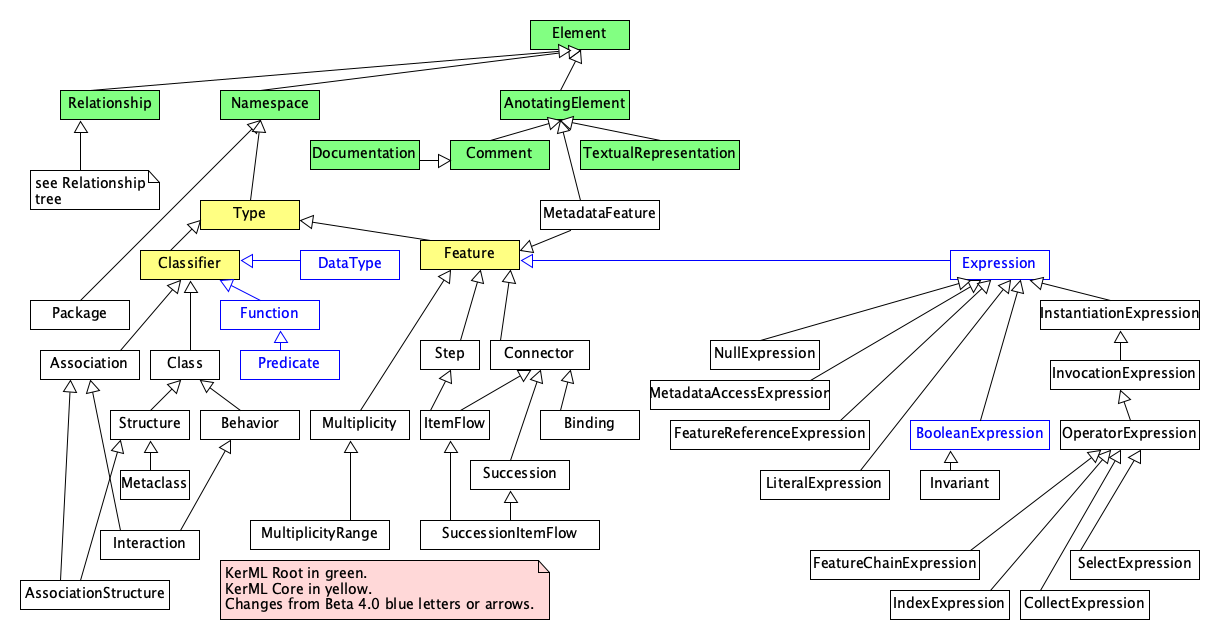
\includegraphics[width=6in]{../pics/KerML-SFS}
\caption{DataType Abstract Syntax}
\label{fig:datatypeabstractsyntax}
\end{center}
\end{figure}

\pn \textbf{validateDataTypeSpecialization:}~~
A \texttt{DataType} must not specialize a \texttt{Class} or an \texttt{Association}.\\
\texttt{ownedSpecialization.general->} \\
\hspace{10pt}~~\texttt{  forAll(not oclIsKindOf(Class) and} \\
\hspace{10pt}~~\texttt{  not oclIsKindOf(Association))}

\pn The class of \texttt{DataType} is the union of Scalar Values (defined in the \texttt{ScalarValues} library), Vector Values (defined in the \texttt{VectorValues} library), and Collections (defined in the \texttt{Collections} library).

Where Data Types are $DT$, Scalar Values are $SV$, Vector Values are $VV$, and Collections are $C$ (whose \texttt{element} features are restricted to $DT$:
\begin{restatable}{definition}{datatype}~\blTitle{df-datatype}~ Define \texttt{DataType}.  
\begin{align}
\vdash DT~=~SV~\cup~VV~\cup~C\label{eq:df-datatype}\tag{df-datatype}
\end{align}
\end{restatable}

\subsection{Scalar Values $SV$:}\label{sec:scalarvalues}

Formal definitions of numeric and boolean values in the \texttt{ScalarValues} library are defined in \ref{sec:sets} and summarized in the table below.
\begin{description}
\item[\texttt{Positive}=$\mathbb{N}$]\index{ natural@$\mathbb{N}$ natural} denotes the set of all natural numbers, excluding 0 \ref{eq:df-nn}; 
\item[\texttt{Natural}=$\mathbb{N}_0$]\index{ natural@$\mathbb{N}_0$ natural} denotes the set of all natural numbers, including 0 \ref{eq:df-n0}; 
\item[\texttt{Integer}=$\mathbb{Z}$]\index{ integer@$\mathbb{Z}$ integer} denotes the set of all integers \ref{eq:df-z}; 
\item[\texttt{Rational}=$\mathbb{Q}$]\index{ rational@$\mathbb{Q}$ rational} denotes the set of rational numbers \ref{eq:df-q};  
%\comment{need to add ref to Q definition}
\item[\texttt{Real}=$\mathbb{R}$]\index{ real@$\mathbb{R}$ real} denotes the set of real numbers \ref{eq:df-r};
\item[\texttt{Complex}=$\mathbb{C}$]\index{ complex@$\mathbb{C}$ complex} denotes the set of complex numbers \ref{eq:df-c};
\item[\texttt{Boolean}=$\mathbb{B}$]\index{ boolean@$\mathbb{B}$ boolean} denotes the set \(\{\top, \bot\}\).\footnote{$\top \equiv$ \texttt{true}; $\bot \equiv$ \texttt{false}} \ref{eq:df-tru}~\ref{eq:df-fal}
\end{description}
For \texttt{String}, $\mathbb{S}$,\index{ string@$\mathbb{S}$ string} use the definition of \texttt{STRING\_VALUE}  in KerML 8.2.2.5.

For \texttt{Time}, $\mathbb{T}$,\index{ time@$\mathbb{T}$ time} specializes \texttt{Real} to be used as the value of time instants is added to $SV$.

\begin{lstlisting}
datatype Time specializes Real;
\end{lstlisting}

%When we say \texttt{at something} that something must be in $\mathbb{T}$.

\begin{restatable}{definition}{scalarvalues}~\blTitle{df-scalarvalues}~ Define \texttt{ScalarValues}.  
\begin{align}
\vdash SV = \mathbb{N} \cup \mathbb{N}_0 \cup \mathbb{Z} \cup \mathbb{Q} \cup \mathbb{R} \cup \mathbb{C} \cup \mathbb{B} \cup \mathbb{S} \cup \mathbb{T} \label{eq:df-scalarvalues}\tag{df-scalarvalues}
\end{align}
\end{restatable}



\subsection{VectorValues $VV$:}\label{sec:vectorvalues}

The \texttt{VectorValues} library provides several handy types in 1, 2, or 3 dimensions by specializing \texttt{Collections\-::Array} and redefining features \texttt{elements} and 
\texttt{dimension}.

\subsection{Collections $C$:}\label{sec:collections}

The \texttt{Collections} library provides several groupings of elements, all specializing \texttt{Collec\-tions::Collec\-tion} having feature \texttt{elements} to define the types of elements it contains.

\comment{All of these can be defined in terms of Metamath extensible structures, but will be messy.  Space for description and \textbackslash ref\{\} provided.}

\begin{description}
\item[\texttt{OrderedCollection} ] 
\item[\texttt{UniqueCollection} ] 
\item[\texttt{Array} ] 
\item[\texttt{Bag} ] 
\item[\texttt{Set} ] 
\item[\texttt{OrderedSet} ] 
\item[\texttt{List} ] 
\item[\texttt{Map} ] 
\item[\texttt{OrderedMap} ] 
\end{description}
All of which can and should be formally defined.

\textbf{\color{red}{However, all \texttt{Collections} are unrestricted to element type.  There must be a constraint \texttt{checkDataTypeElement} to make sure that any elements used are themselves in $DT$.}}

\pn \textbf{checkDataTypeElement:}~~ The \texttt{element} of a \texttt{Collection} must specialize \texttt{DataValue}.\\
\texttt{element->specializesFromLibrary('Base::DataValue')}
